%
% you should only have one "documentclass" line.  the following lines
% are samples that give various options.  the nofrontmatter option is
% nice because it suppresses the title and signature pages when you want
% to focus only on the main body of the thesis
%
% Friday April 10 2010 Ray Hylock <ray-hylock@uiowa.edu>
% documentclass options:
%   abstractpage            if you want to add an internal abstract (optional)
%   ackpage                 if you would like to add an acknowledgements page (optional)
%   algorithms              if you want a list of algorithms (optional)
%   appendix                if you have an appendix (optional)
%   copyrightpage           if you wish to copyright your thesis (optional)
%   dedicationpage          if you wish to make a dedication (optional)
%   epigraphpage            if you would like to add an epigraph to the beginning of your thesis (optional)
%   examples                if you want a list of examples (this uses the ntheorem package)
%   exampleslemmas          if you want a combined list of examples and lemmas (this uses the ntheorem package) (optional)
%   examplestheorems        if you want a combined list of examples and theorems (this uses the ntheorem package) (optional)
%   exampleslemmastheorems  if you want a combined list of examples, lemmas, and theorems (this uses the ntheorem package) (optional)
%   figures                 if you have any figures (this is required if you have even one figure)
%   lemmas                  if you want a list of lemmas (this uses the ntheorem package) (optional)
%   lemmastheorems          if you want a combined list of lemmas and theorems (this uses the ntheorem package) (optional)
%   nofrontmatter           suppresses the title and signiture pages for working on the body
%   tables                  if you have any tables (this is required if you have even one table)
%   theorems                if you want a list of theorems (this uses the ntheorem package) (optional)
%   phd                     if phd student; this will add the doctoral abstract (mandatory for PhD and DMA thesis candidates only)
%

% full options
%\documentclass[phd,abstractpage,copyrightpage,dedicationpage,epigraphpage,ackpage,figures,tables,lemmas,appendix]{uithesis}

% common options
%\documentclass[phd,dedicationpage,ackpage,figures,tables,appendix]{uithesis}

% example
\documentclass[phd,appendix,figures]{uithesis}

%=============================================================================
% User packages
%=============================================================================
\usepackage{bookmark}	% [recommended] for PDF bookmark generation
\usepackage{blindtext} 	% example text generation
\usepackage[ruled,chapter]{algorithm}  % display algorithms
\usepackage[super,comma,sort,numbers]{natbib}
% to place figures/subfigures
\usepackage{graphicx}
\usepackage{subfig}
% path to figures
\graphicspath{{img/Aim1/}{img/Aim2/}{img/Aim3/}{img/CurrentStudy/}{img/GeneralDiscussion/}{img/GeneralMethods/}{img/Introduction/}}
\usepackage{forloop} % for loops display images
\usepackage{hyperref} % to insert hyperlinks
\usepackage{textcomp} % to write degree symbols
\usepackage{float} % image placement
% for smaller captions
\usepackage[labelfont=bf]{caption}
\captionsetup{font=footnotesize}
% https://tex.stackexchange.com/questions/370278/is-there-any-reason-to-use-inputenc
\usepackage[utf8]{inputenc} % for non-ascii characters

%=============================================================================
% prelude
%=============================================================================

\title{Task Related Correlations}
\author{James Kent}
\dept{Neuroscience}

% multipleSupervisors=true for two advisors
\setboolean{multipleSupervisors}{false}
\advisor{Assistant Professor Dr. Michelle Voss}
% for multiple advisors; change <value> to line up the names
%\setboolean{multipleSupervisors}{true}
%\advisor{Advisor 1\\\hspace{<value>mm}Advisor 2...}
%
% edit the names below to have your committee members names appear
% on the signature page.  memberOne should be your advisor.
%
\memberOne{Michelle Voss}
\memberTwo{Eliot Hazeltine}
\memberThree{Vincent Magnotta}
\memberFour{Jatin Vaidya}
\memberFive{Jan Wessel}
\submitdate{May 2020}
\copyrightyear{2020}

\Abstract{
\blindtext
}

%\dedication{Dedication here (optional)}

%\epigraph{Epigraph here (optional)}

%\acknowledgements{Acknowledgements here (optional)}

\begin{document}

\frontmatter

%=============================================================================
\chapter{Introduction}
%=============================================================================
What is it that makes us human? 
What makes us better than automatons that blindly react to their environment?
Some may say free will, but perhaps a better answer is cognitive control.
Cognitive control is the ability to take into account contextual cues (either previously or currently in your environment) to decide what behavioral route to take in response to a stimulus. 
A common example is driving.
If you are driving through a neighborhood with notoriously short yellow lights, I would hope you are more likely to stop when you see a light turn yellow.
If instead, you are driving through a neighborhood where the yellow light lasts for eight, maybe even ten seconds, you may cruise right through the intersection knowing you have plenty of time.
The two automaton behaviors are the braking and continuing (maybe speeding up a little) through the yellow light.
Cognitive control represents the process that selects one of the two behaviors.
In this example, cognitive control is being informed by the spatial location and its association with either a short or long yellow light.

There is a vast sea of research about cognitive control, its ontology, its neural basis, and when it breaks down, but several key gaps still remain ~\citep{Gratton2017,Dosenbach2010,Braver2000}.
\textbf{The first key gap is how neural networks are represented during a task that requires cognitive control}.
The current literature goes on at length about activation studies and meta-analyses, as well as clever mixed-design (event \& block) experiments ~\citep{Gratton2017a,Lerman-Sinkoff2017,Herd2006,Rizio2012,Cooper2015,AppelBaum2014}.
There are even reports of what networks are a part of cognitive control using resting state data ~\citep{Dosenbach2007}.
However, the crucial missing evidence is directly observing the networks during a task.
There are several technical reasons why network organization hasn't been investigated during a task and this current proposal seeks to overcome the technical difficulties and provide an open source tool for others to use.
Filling this gap will provide direct evidence that cognitive control networks exist during performance of a task and provide a more solid foundation for studying networks related to cognitive control in the future.

\textbf{Second is how the neural networks relate to behavior in cognitive control tasks}.
Again, clever experiment designs, lesion studies, and task manipulations have related changes of activity to cognitive control and behavior, but there is still no evidence directly linking the level of task network connectivity to task behavior ~\citep{Nomura2010,Egner2004,Gonthier2016a,Braver2010,Huang2017}.
The present research seeks to fill this gap and provide a more definitive connection between proposed cognitive control networks and behavior.

Behavior has now been mentioned several times, but how is cognitive control measured in the lab?
Using the driving example, behavior is measured by whether the person stops or speeds through the intersection when the light is yellow.
In the lab, we don't use cars and pedals, we use pictures.
Specifically, there are a class of tasks that tap in the construct of cognitive control, and these include, but are not limited to: Stroop, Eriksen Flanker, and Simon ~\citep{Simon1967,Eriksen1974a,Stroop1935}.
In all of these tasks, there is a dominant, automatic response and a weaker controlled response. 
For a word version of the Stroop task, the automatic response is reading the word.
For an arrow Flanker task, the automatic response is pressing the button corresponding to the predominant direction of the arrows.
For the Simon task, the automatic/dominant response is responding with the hand that is closest to the stimulus shown on the screen.
The controlled/weaker action for each of the tasks are: reporting the color of the font, responding to the direction of only the middle arrow, and responding with the hand the stimulus is associated with, respectively.
Sometimes the automatic response is congruent with the controlled response (e.g. the word red has a red font color), but other times the response is incongruent (e.g. the word red has a blue font color).
For the incongruent trials, the controlled response is different from the automatic response, and this introduces conflict.
Thus, by looking at the reaction time difference between incongruent trials and congruent trials, we are peering into the cost associated with engaging cognitive control to override an automatic response (however, there are alternative explanations) ~\citep{Hommel2011}. 

Correlating network intra-connectivity with reaction time cost across participants (e.g. one measure per participant), a direct relationship between cognitive control networks and behavior will be established.
This research will quantitatively connect the theoretical notions of cognitive control proposed by Braver, and the anatomical basis of cognitive control derived primarily from Dosenbach ~\citep{Braver2008,Dosenbach2007}

\section{History of Cognitive Control}

To understand cognitive control, we must first take a step back to understand the theories that connected an individual's environment with their responses, presumably through the 3 pound piece of pulsating meat between our ears.
The 1960s were a tumultuous time of drugs, protests, and revolutions. 
Not to be outdone by the social and political environments, psychology staged its own revolution, a cognitive revolution against a backdrop of behaviorism, although the concept of revolution may be romanticizing what actually happened ~\citep{Leahey1992}. 
The gelatinous black box of the brain needed to be unveiled, and cognitive psychology was determined to pull back the curtain. 

One of the first cognitive models to gain traction during the "revolution" was Sternberg's serial processing model.
As the name suggests, Sternberg's serial processing model suggested people processed stimuli one at a time, serially, which gave psychology groundbreaking concepts such as the primacy and recency effects ~\citep{Sternberg1966}.

However, as with all models, serial processing was inadequate in explaining the flexibility of human cognition.
Namely, the deficit was the thought that human cognition was treated as an open loop system, where information was processed in stages and produced behavioral output. 
While closed-loop systems were pervasive in the subfield of cybernetics, the idea did not really pierce the veil of psychology until 1970 when Gregory published about the distinction between top-down and bottom-up processing ~\citep{Gregory1970}.
With the knowledge that people behave differently to the same stimulus depending on the context, psychologists concluded that in addition to feed-forward processing, there must also be a feedback mechanism to inform the appropriate response ~\citep{Gregory1970}.
The seed of cognitive control was planted.

Following this line of thought, Shriffrin \& Schneider differentiated the top-down and bottom-up processes, otherwise known as controlled and automatic processes by looking at processing speed, attentional load, and capacity ~\citep{Shiffrin1977}. 
They derived three basic attributes of cognitive control. One, controlled processes are slower relative to automatic processes. 
Two, controlled processes are in competition with automatic processes. 
And three, controlled processes tap into a shared limited resource.

The next major model of cognition that involved feedback (controlled processing) was Norman and Shallice's (1986) supervisory attentional system (SAS) ~\citep{Norman1986}. 
The SAS encompasses slow, deliberate top-down processes when pursuing the habitual response is incorrect or inadequate.
Around the same time Baddeley released a model of working memory which included a Central Executive where putative functions of cognitive control would be performed ~\citep{Baddeley1996}.
However, as Baddeley noted himself, his concept of the central executive was too vague and could only "serve as little more than a ragbag" (p.6). 
Researchers have found this ambiguous cloud of higher cognition within the central executive, but efforts to divide it up into useful chunks has evaded strong empirical scrutiny for years.

Miyake et al. (2000) tackles the central executive head on and began carving the construct into distinct components. 
Their group found that executive function could be split into three categories:
1) shifting between tasks or mental sets,
2) updating and monitoring of working memory representations, and
3) inhibition of dominant or prepotent responses ~\citep{Miyake2000}.
This work was instrumental towards providing a stronger behavioral definition of cognitive control, and paved the way for well designed imaging studies to study cognitive control.
Miyake provided an excellent first-pass into dividing up the central executive, but more detailed explanations are needed.
For example, the congruency sequence effect (i.e. Gratton effect) would require monitoring of working memory representations and inhibition of a dominant response in favor of a less dominant response, but do these processes occur over the course of the task between stimulus presentations, or perhaps they are engaged when the stimulus is presented, or perhaps a mixture of both?

Braver added a much needed explicitness and computational validity to cognitive control. With his detailed, testable models, Braver began to peer into the conceptual void of the central executive and its anatomical underpinnings ~\citep{Braver2001}. 
He proposed a gating model, where phasic dopamine release in the prefrontal cortex (PFC) allowed for flexible updating of the active memories being held in place.

To illustrate, imagine a color stroop task where the participant has to name the color of the font, and ignore the word that is printed.
The foundation of the stroop task assumes that reading is an automatic process that requires little to no control, whereas naming the color is a controlled process that can act in opposition to reading if the printed word is also a color (e.g. the word blue colored in red font).
The maintenance of the goal (name the font color, not the word) is held in working memory (in the PFC), and the ability to acquire and maintain this goal is hypothesized to be a result of phasic dopamine release. 
If there was a long sequence of congruent trials (e.g. the word red with the font color red), the participant may take a shortcut and use the automatic process of naming the word.
An incongruent trial may appear after this sequence of congruent trials, and then the participant has to engage the controlled process through phasic dopamine release into the PFC.
Again, a common thread of these models does not lay with their accuracy to describe all of human cognition, but with their utility to frame our thoughts and describe particular aspects of human cognition. 


\section{Dual Mechanisms of Control}

As mentioned in the previous section, an additional layer of nuance emerges when one asks exactly when is cognitive control engaged.
Is cognitive control engaged when the stimulus/probe appears or is it maintained over the course of the task?
Does it matter?
Is it all a part of the same process?
Braver has classified the above circumstances as different forms of cognitive control, reactive and proactive, and they form the Dual Mechanisms of Control (DMC) framework ~\citep{Braver2012}.
A way to conceptualize proactive and reactive control is early selection and late correction, respectively ~\citep{Jacoby1999}.
Early selection means the goal is held in working memory either for the duration of the task, and/or the period between a cue and a probe.
Late correction, on the other hand, means the goal is not held in working memory, rather, the decision about whether the automatic or the controlled behavior set should drive behavior is not engaged until a probe or stimulus is seen.
Braver found this behavioral distinction between proactive and reactive cognitive control while working on the AX version of the continuous performance task (AX-CPT) ~\citep{Paxton2008}.
The AX-CPT is a task where participants are to respond to a particular cue-probe pair, namely A-X.
All other cue-probe pairs (A-Y, B-X, B-Y) should be ignored and the participant should not respond to the probe on those trials.
This task becomes difficult because the A-X trials occur with a high probability (e.g. 70\%) developing an expectancy to respond to this cue-probe pair.
Following this built up expectancy, two other cue-pairs become interesting, A-Y and B-X.
Participants may have built up an expectancy to respond to a probe after the target cue A, and/or built up an expectancy to respond to probe X even if it was preceded by a B cue.
The B-Y trials act as a control because there is no bias present in the cue or the probe to tempt the participant to respond incorrectly.
This task lends itself towards clear predictions of performance depending an individual is particularly engaging proactive or reactive cognitive control.
Specifically, if a participant was using a more proactive strategy or in other words, were using strong goal maintenance, we would expect to see improved B-X performance, but a diminished A-Y performance.
On the other hand, participants with impaired goal maintenance would be expected to perform reactively, showing poorer performance on the B-X trials relative to the A-Y trials ~\citep{Paxton2008}.

What populations may have poor goal maintenance?
One widely studied population, by Braver and others is healthy older adults.
Through Braver's proposed mechanism of less reliable dopamine signaling and poorer frontal lobe performance, the consequence of impaired goal maintenance is an increased reliance on reactive cognitive control, even in circumstances where proactive control would lead to better performance.
While this description of proactive and reactive cognitive control may lead one to believe that they are two ends on the same spectrum, the proposed separate neural architecture and recent behavioral evidence suggest they are semi-independent processes ~\citep{Gonthier2016}.
The difficulty in demonstrating their independence lays within producing a double dissociation.
Schizophrenia and aging provide excellent models of proactive control breaking down, but there is not currently a model for the break down of reactive control in behavior that preserves proactive cognitive control.
Thus while one could theoretically use both proactive and reactive cognitive control, in practice the evidence suggests the engagement of proactive control results in a lesser need to engage reactive control ~\citep{Gonthier2016a}.
Taking the perspective that control is costly in terms of effort and neural resources, using both reactive and proactive control mechanisms strongly is wasteful.

\section{Neural Basis of Cognitive Control}

Akin to Ralphie's excitement when he got his Red Ryder air rifle, the world of neuroscience was abuzz with the advent of fMRI in 1990 ~\citep{Ogawa1990}. 
The ability to observe the inner machinations of the mind without costly surgeries and reliance on clinical populations greatly expanded the granularity of inquiry researchers were eager to ask. 
This was a boon for cognitive control as well because of the theoretical ambiguities outlined in the previous sections about the central executive.
Where is the center of control, could one point it out in a brain scan, or was it perhaps more complicated?
Cognitive Control saw its first debut in fMRI in 1995 with D'Esposito's search for the Central Executive ~\citep{DEsposito1995}. 
While Cognitive Control was not in the lexicon at the time of publishing, the markers for its existence were there in the prefrontal cortex.

Parallel to Braver's work, Dosenbach released a theoretical framework of cognitive control named dual mechanisms of cognitive control ~\citep{Dosenbach2007}. 
This model contained a quick/adaptive component and a longer sustained component.
Sound familiar?
Braver's conception of proactive and reactive cognitive control maps onto the slow sustained component and the quick/adaptive component, respectively ~\citep{Braver2012}.
The proactive component is anchored by the dorsal anterior cingulate cortex and anterior insula in the cingulo-opercular network ~\citep{Dosenbach2008}.
The reactive component is anchored by the lateral prefrontal cortex and the parietal cortex in the fronto-parietal network ~\citep{Dosenbach2008}.
A double dissociation between the fronto-parietal and cingulo-opercular networks has been demonstrated in a lesion study, providing further evidence of the network separability ~\citep{Nomura2010}.
While Braver has mentioned Dosenbach's analytical methods, serious inquiry mapping the relationship between proactive and reactive control with the fronto-parietal and congulo-opercular networks has yet to be established ~\citep{Braver2006,Cooper2015}.

\section{Intrinsic and Extrinsic Networks}

In the past decade and currently, accumulating evidence suggests intrinsic activity (i.e. what goes on in your brain when you aren't performing a task) is more than physiological noise and contributes meaningfully to behavior ~\citep{Busch2010,Kenet2003,McCormick1999,Mateo2017}.
This field of "resting state" imaging has established itself as a measure in the fMRI world that is likely not going away any time soon ~\citep{VandenHeuvel2010,Shen2015}.
Resting state imaging measures the spontaneous blood flow that occurs in the brain in the absence of a task.
Blood flow in some regions tend to co-occur with blood flow in spatially disparate regions, creating "functional" connectivity as measured through Pearson's Correlations or other connectivity measures.
Connectivity measures between regions (or between multiple regions known as networks) have been correlated with traits and behaviors with success ~\citep{Dennis2011,Duchek2013}.
Intervention studies have also seen changes in connectivity in relation to the behavior that was targeted ~\citep{Horowitz-Kraus2015}.
Some researchers attribute the functional connections between regions to Hebbian mechanisms, in which a simple interpretation is that "regions that fire together wire together" ~\citep{Harmelech2013}.
Thus if there is a long history of regions robustly communicating with each other, then we would be able to see that relationship represented in resting state.
However, there are many other sources that may contribute to resting state signal, such as motion, heartrate, non-neuronal processes, etc. ~\citep{Winder2017,Murphy2013}.

Given the multiple non-neurological sources of signals in resting state, another way to "boost" the signal of relevant networks is to observe them during a task ~\citep{Cole2014}.
In Cole (2014) they found increased connectivity in the fronto-parietal network from the task data, however in their model, they did not remove the impact of trial-to-trial variability, suggesting that the increased fronto-parietal connectivity could have been due to stimulus evoked connectivity and not due to a general state difference between rest and task.
The current study will use one regressor per trial to model residual connectivity, effectively removing the trial to trial variation the Cole (2014) modeling strategy left in.
Residual connectivity will measure the intrinsic connectivity and the additional task demands that are not directly related to the stimulus such maintaining goal information.
Thus residual connectivity represents both intrinsic and extrinsic network properties.

Beta-series, which measures the trial-to-trial variation of the brain's response to stimuli, mainly represents the extrinsic network, that is, connectivity induced by stimuli. ~\citep{Rissman2004}.
The trial-to-trial variance may also be influenced by intrinsic spontaneous fluctuations of the BOLD response that is ongoing throughout the task, and introduce correlations that are not directly related to seeing the stimulus ~\citep{He2013}.
However, as the Cole (2014) study found, the stronger fronto-parietal intra-network connectivity is likely due to the trial-to-trial variations of the BOLD response to stimuli.
The currently proposed study will interrogate this difference and provide a clearer contribution of stimulus evoked connectivity (beta-series) and residual connectivity.


%=============================================================================
\chapter{The Research}
%=============================================================================

Advances in both fMRI analysis and theory of cognitive control have collided to produce ripe new areas to advance our understanding of cognitive control through fMRI ~\citep{Braver2012,Rissman2004,Mumford2012,Cisler2012}.
We can find evidence of cognitive control in our daily lives, from switching between an email and a conversation to making a quick decision behind the wheel. 
Specifically, cognitive control refers to the ability to use our context to inform our decisions. Cognitive control can be broken down into two modes, proactive and reactive ~\citep{Braver2012}. 
Proactive cognitive control encompasses the conflict preparation processes that occur for the entire duration of a task, and/or the conflict preparation between a cue and a stimulus.

In other words, the conflict processes that are not in direct response to a stimulus.
Reactive cognitive control, on the other hand, refers to the conflict adaptation that happens directly in response to a stimulus.
Two separable networks have been identified in proactive and reactive cognitive control, the cingulo-opercular (proactive) and fronto-parietal (reactive).
However, to this author's knowledge, there does not exist any research demonstrating the connectivity of these networks during a cognitive control task in fMRI.
Thus, the main thrust of this research is to establish these networks during a cognitive control task using two analytical methods theoretically sensitive to reactive or proactive cognitive control.

\begin{figure}[H]%
    \centering
    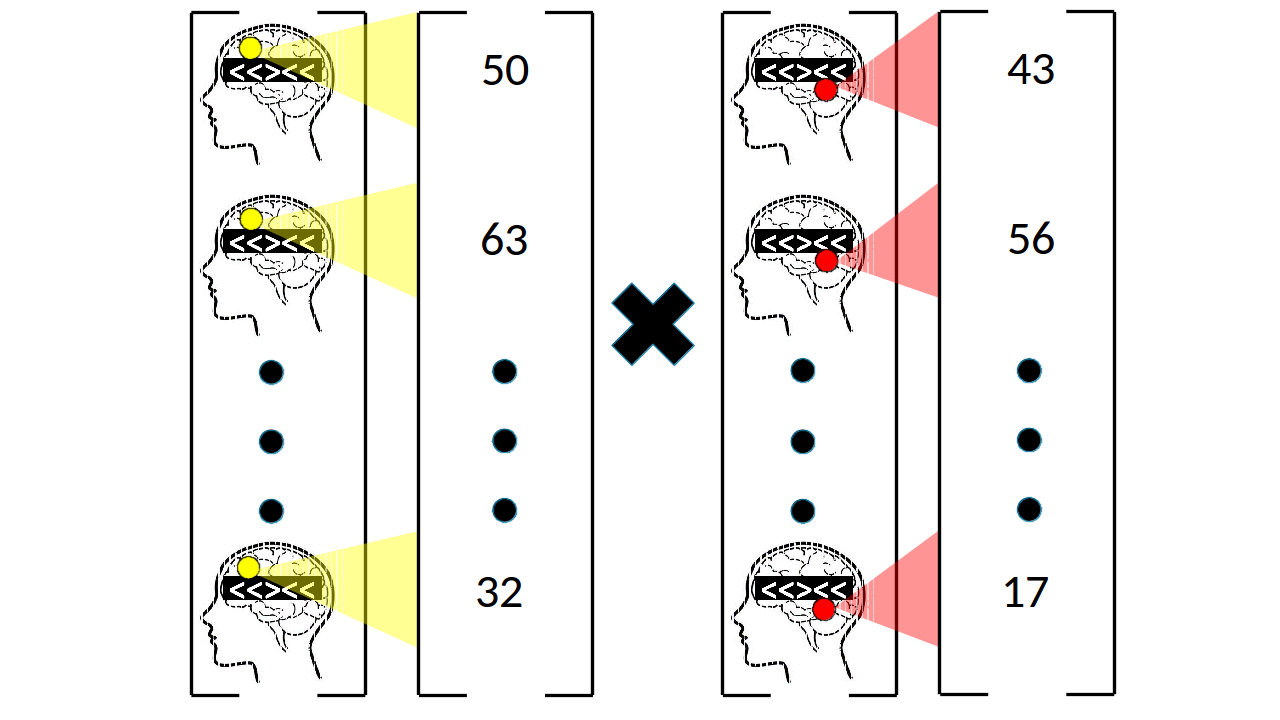
\includegraphics[scale=0.25]{betaseries_correlation_illustration}
    \caption{Setting up Beta-series Correlations. In the flanker task example above, betas (i.e. activation index) have been fit to every voxel per trial, and separated by condition (incongruent and congruent). This figure is only representing the incongruent trials, but both incongruent and congruent trial data can be collected. Regions of interest (ROIs) can be selected from these beta-maps and all the voxels within the ROI are averaged. Once the betas are extracted from each ROI for each trial, the resulting lists of betas can be correlated with each other.}%
    \label{fig:betaseries_correlation_illustration}%    
\end{figure}

The first method is beta-series correlations and is sensitive to the theoretical notion of reactive cognitive control (Figure ~\ref{fig:betaseries_correlation_illustration}). 
Beta-series correlations model the response after a congruent or incongruent stimulus capturing the "on-the-fly" conflict adaptations, otherwise known as reactive cognitive control.
Aim 1 will establish the use of this method due to its novel application to fast-event related designs of fMRI.

The second method is residual correlations; the time-course of the brain's activity after regressing out the stimulus onset information ~\citep{Fair2007,Cole2014,Bolt2017}. 
Residual correlations measure the theoretical notion of proactive cognitive control because proactive cognitive control represents the stable maintenance of goal-relevant task information throughout the performance of the task, which is what the time-series will represent.
Behavioral measures of proactive and reactive cognitive control exist, however outside of the AX-CPT it is difficult to analyze purely proactive and reactive behavioral components. 
Following the characterization of the purported reactive and proactive cognitive control networks, their relationship to existing behavioral measures will be established.
This research will contribute to the ongoing conversation of the neural basis of cognitive control, and provide a more direct metric of these networks during a  cognitive control task.

\section{Specific Aims}
\begin{figure}[H]%
	\centering
	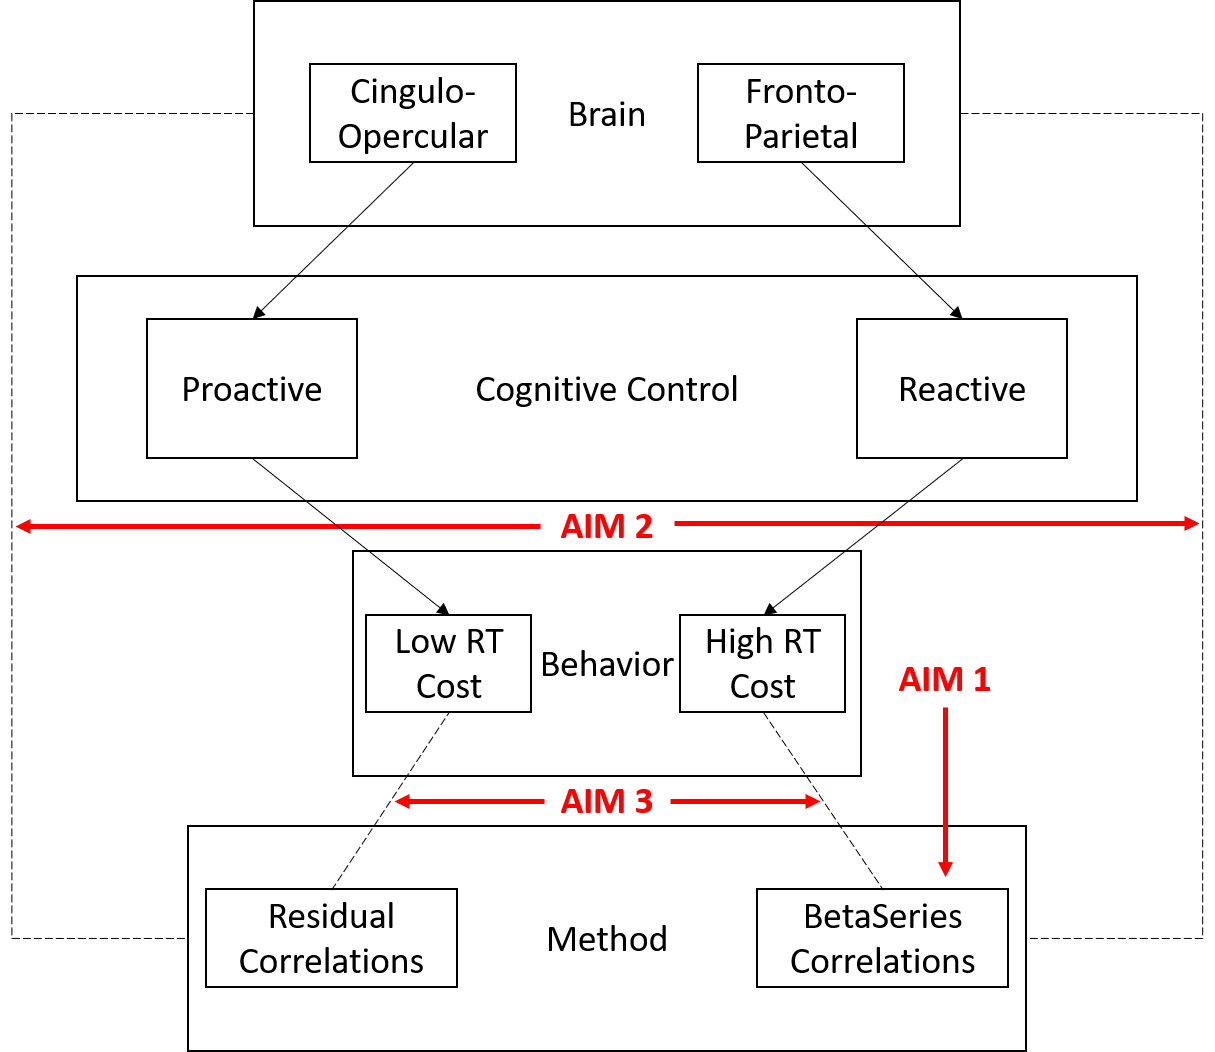
\includegraphics[width=1\linewidth]{all_aims}
	\caption{Outline of my three aims. Aim 1 seeks to produce and validate software developed with nipype to perform beta-series correlations. Aim 2 will profile beta-series correlations and residual correlations on the same task datasets to derive differences and similarities between the methods. Finally, Aim 3 connects the correlations derived from the two methods and compares them to behavioral measures of cognitive control (e.g. reaction time cost). Abbreviations: RT=reaction time}
	\label{fig:all_aims}
\end{figure}

\textbf{Specific Aim 1}: Create and validate a program to perform beta-series correlations
\newline
\textit{Rationale}: A beta in this context refers to the free varying parameter in the general linear model (GLM) that "fits" the data.
\begin{equation} \label{eq:1}
Y = X\beta + \epsilon 
\end{equation}
Equation \ref{eq:1} is the basic GLM where $Y$ represents the time-series we are attempting to explain. The $\beta$ assumes any value that minimizes the squared error between the modeled data and the actual data. 
$\epsilon$ refers to the error that is not captured by the model.
\begin{equation} \label{eq:2}
Y = X_{Ti}\beta + \epsilon
\end{equation}
Equation \ref{eq:2} describes the least squares separate (LSS) implementation of a GLM, where the major difference is in the design term $X_{Ti}\beta$.
This notation represents that a particular trial's $\beta$ is being estimated and not the average of all the trials.
Another detail not explicitly noted in the equation is that all other trials (e.g. every trial except the one being modeled) are treated as a single nuisance regressor, so the beta will only account for the unique variance described by that trial and any shared variance will given to the other trials.
Thus we can account for the unique trial-to-trial variability of the betas.
\begin{algorithm}
	\caption{Beta-series Algorithm}\label{al:1}
	\begin{algorithmic}[1]
		\FOR{\texttt{Ti in Trials}}
    		\STATE \texttt{$Y = X_{Ti}\beta + \epsilon$}
		\ENDFOR
	\end{algorithmic}
\end{algorithm}
The algorithm to calculate each trial's $\beta$ estimate will be iteratively performed across trials and depending on the trial's condition (e.g. congruent vs. incongruent), the $\beta$ value will be placed in its corresponding list (Algorithm ~\ref{al:1}).
While programs exist to compute beta-series correlations, there isn't one that utilizes least squares separate estimation, a modeling strategy that would help with deriving betas from fast event related designs with beta-series correlations ~\citep{Mumford2012,Gottlich2015}. 
The proposed software seeks to fill that gap (Figure ~\ref{fig:all_aims}).
\newline
\textit{Hypothesis}
The beta-series software will produce data that will generate coherent correlative networks.
These networks will be spatially similar to published existing networks ~\citep{Smith2009,Dosenbach2010}
\newline
\textit{Method}: Under the Nipype framework, I will primarily use FMRIB's FSL utilities to model data on a trial-by-trial basis ~\citep{Smith2004,Gorgolewski2017}. 
Using a traditional GLM with a double gamma basis function, modeling will be completed by performing a GLM for each trial individually, with all other trials combined into a single term to form a regressor of non-interest ~\citep{Mumford2012}.

Validation of the beta-series software will be performed on two younger adult datasets where they performed a standard arrow flanker task (slow event related) or a simon task (fast event related).
Two methods of analysis will be used to validate the beta-series approach, Independent Components Analysis (ICA), and ROI-ROI correlations with 160 ROIs derived from Dosenbach's meta-analysis of task data ~\citep{Dosenbach2010}.

ICA will reveal the underlying structure of the data, and the resulting components will be spatially correlated with existing parcellations using ICA ~\citep{Smith2009}(Figure ~\ref{fig:smith_maps}).
Medium to large spatial overlap (r $>$ .25) was found significant in smith (2009) and a similar threshold will be used to identify the fronto-parietal and cingulo-opercular networks.

ROI-ROI correlations will provide further evidence that beta-series networks cluster together. Each participant will have a 160 x 160 matrix of Pearson's R correlations, with each ROI's network affiliation being labeled by Dosenbach (2010) (Figure ~\ref{fig:dosenbach_rois}). 
Within network correlations will be generated along with between network correlations, producing two values for each participant (average within network correlation and average between network correlation).
Then a one-tailed student's t-test will evaluate whether the within network correlations are significantly greater than between network correlations.
\newline
\textit{Alternative Methods}: If the beta-series approach introduces bias into the correlation measures (e.g. all regions are strongly correlated with each other), the method to derive betas will be re-evaluated.
If there is not a suitable method to reduce/remove the bias, psycho-physiological interactions (PPI) may be used instead to derive relative trial activation, although there is no a priori reason to believe PPI will be less susceptible to bias.
If network parcellations do not reasonably overlap with existing parcellations, this could be of interest by itself.
It may suggest novel networks are generated during a task that do not exist in identified resting state networks.
However, to draw a relation with the existing literature, specific ROIs from the major network hubs (Dosenbach, 2010) will be used to give the beta-series correlations their best shot at overlapping with existing networks.
If the ROI-ROI correlation, student's t-test does not provide enough rigor to demonstrate the within versus between network connectivity, graph theoretical measures such as the participation coefficient and within-module degree will be used to identify provincial hubs and connector hubs ~\citep{Wang2010}. 
\newline
\textbf{Specific Aim 2}: Characterize the relationship between beta-series correlations (reactive) and residual correlations (proactive) during cognitive control tasks.
\newline
\textit{Rationale}: The dual mechanisms of control theory posits these networks should be differentially sensitive to the type of correlation method applied ~\citep{Dosenbach2007,Braver2006}. 
In the existing literature there has not been an attempt to analyze data with these  complementary methodologies, presenting an excellent opportunity to conceptually frame task data into stimulus evoked components and persistent background components.
\newline
\textit{Hypothesis}:
With residual correlations, the connectivity within the cingulo-opercular network should be stronger than the connectivity within the fronto-parietal network. With beta-series correlations, the connectivity within the fronto-parietal network should be stronger than the connectivity within the cingulo-opercular network.
\newline
\textit{Methods}: To calculate residual correlations two steps will be completed.
First the stimulus responses will be modeled and removed from the data.
Second the data will be z-transformed and Pearson's R correlations will be performed.
Stimulus onsets from the task will be represented as impulses and convolved with a double gamma function to be used as the basis function for the GLM. 
Each stimulus event will entered into the GLM as its own regressor.
This ensures the trial-to-trial variance will be removed from the task data, and not just the mean response of there being a stimulus. 
The residual data from the GLM will represent BOLD responses not captured by direct responses to stimuli. 
Subsequently, the residuals will be z-transformed to normalize the distributions and Pearson's correlations will be extracted from ROIs that participate in the fronto-parietal network and the cingulo-opercular network.
The beta-series calculation will be performed as described in aim 1. 
The correlation will be performed in the same manner as described for the residual calculations with an extra step for cognitive subtraction.
That is, instead of residuals, the beta-maps will be normalized and ROI-ROI correlations will be performed for both congruent and incongruent conditions.
The extra step will be a subtraction (incongruent - congruent) of the Pearson's R correlation matrices, signifying regions that are more strongly correlated in the incongruent condition relative to the congruent condition.
Average within network correlations will be performed for the cingulo-opercular and fronto-parietal networks across participants for both beta-series and residual correlations.
Then student's t-tests will be performed, with hypothesized directional effects for beta-series: fronto-parietal $>$ cingulo-opercular, and residual: cingulo-opercular $>$ fronto-parietal.
\newline
\textit{Alternative Methods}: 
One point of potential weakness is the subtraction method for the beta-series correlations.
There is a possibility correlations between rois do not change significantly between task conditions (e.g. congruent versus incongruent). 
Thus, an alternative may be to collapse the conditions and more generally report the reactive cognitive control response to any stimulus instead of stimuli that invoke strong cognitive control processes.
If the student's t-tests between average within network correlations do not produce results, ICA can be run on both the beta-series and residual maps to produce data driven components for the fronto-parietal and cingulo-opercular networks. The spatial overlap between the components derived from beta-series and from the residual maps will be used to derive ROIs.
\newline
\textbf{Specific Aim 3}: Characterize the relationship between the derived cognitive control networks and established behavioral measures of cognitive control.
\newline
\textit{Rationale}: The fronto-parietal and cingulo-opercular networks are theoretically motivated to explain different aspects of behavior, namely reactive and proactive cognitive control, respectively. 
There is recent work deriving measures from reaction time and dividing the measures into reactive and proactive components ~\citep{Fassbender2014}.
Similarly, there is a growing body of behavioral research designing task paradigms to explicitly divide the behavior into proactive and reactive components ~\citep{Gonthier2016,AppelBaum2014}.
However, this explicit connection of behavior with beta-series and/or residual correlations has not been performed and will fill an explanatory gap towards the relation between cognitive control networks and behavioral engagement of cognitive control.
\newline
\textit{Hypothesis}: The fronto-parietal network derived from the beta-series approach should correlate with the "reactive" components of behavior and the cingulo-opercular network should correlate with the "proactive" components of behavior.
\newline
\textit{Methods}: Behavior will be measured by looking at the congruency effect (e.g. incongruent - congruent) reaction time.
Studies that have manipulated the proportion of congruent/incongruent trials in a task  found a larger congruency effect in blocks in which there were more congruent trials relative to incongruent trials ~\citep{AppelBaum2014,Funes2010}.
This indicates that a larger congruency effect suggests a more reactive strategy, where a late stage correction during the incongruent trials results in a larger reaction time relative to the automatic congruent trials.
On the other hand, a smaller congruency effect suggests a more proactive strategy, if early selection keeps the goal task in mind, the reaction time on the congruent trials may be slower and the incongruent trial reaction times will be faster.
The congruency effect will be measured for each participant, as well as the intra-network connectivity measures for fronto-parietal and cingulo-opercular for both beta-series and residual correlations as explained in aim 2.
The connectivity measures will be correlated with the congruency effect across participants.
\newline
\textit{Alternative Methods}: The congruency effect is one of many analytical methods to parse behavioral data.
Another potentially fruitful method is the congruency sequence effect (i.e. Gratton effect) which states that the trial sequence congruent/incongruent will result in a larger reaction time for the incongruent trial relative to the sequence incongruent/incongruent ~\citep{Gehring1992,Egner2007}.
The difficulty of congruency sequence effects rests in its interpretation under the proactive/reactive framework.
A person with a large congruency sequence effect could be interpreted as utilizing proactive control since they use the previous trial to prepare or adjust proactively to the current trial.
Just as easily, a small congruency sequence effect could be interpreted as utilizing proactive control since the participant must be monitoring the goal information in a proactive manner such that the context in which they see an incongruent trial does not matter.
Another method is look at reaction time variance across conditions ~\citep{Fassbender2014}. 
A large variance difference in reaction time between congruent and incongruent trials (i.e. incongruentVariance $-$ congruentVariance) suggests more lapses in attention, indicating the late-correction reactive control was engaged.
Whereas a small variance difference suggests consistent focus throughout the task, potentially indicating a proactive approach.



%=============================================================================
\appendix
%=============================================================================

%=============================================================================
\chapter{Sample Appendix}

\section{Appendix One}
\blindtext

\section{Appendix Two}
\blindtext

%=============================================================================
\chapter{Another Appendix}

\section{Appendix Three}
\blindtext


%=============================================================================
% bibliography
%=============================================================================
\interlinepenalty=10000	% prevents bib items from splitting across pages
\bibliographystyle{uithesis}
\bibliography{library} 

\end{document}

% currently unused text
\section{General Methods}
Results included in this manuscript (and results to be included) come from preprocessing performed using FMRIPREP version 1.0.4, a Nipype based tool ~\citep{Esteban2018,Gorgolewski2011,Gorgolewski2017}. 
Each T1 weighted volume was corrected for bias field using N4BiasFieldCorrection v2.1.0 and skull-stripped using antsBrainExtraction.sh v2.1.0 (using OASIS template) ~\citep{Tustison2010}. 
Cortical surface was estimated using FreeSurfer v6.0.0 ~\citep{Dale1999}. 
The skull-stripped T1w volume was co-registered to skull-stripped ICBM 152 Nonlinear Asymmetrical template version 2009c using nonlinear transformation implemented in ANTs v2.1.0 ~\citep{Avants2018,Fonov2009}.
Functional data was slice time corrected using AFNI and motion corrected using MCFLIRT v5.0.9 ~\citep{Jenkinson2002,Cox1996}. 
This was followed by co-registration to the corresponding T1-weighted volume using boundary based registration 9 degrees of freedom - implemented in FreeSurfer v6.0.0 ~\citep{Greve2009}.
Motion correcting transformations, T1 weighted transformation and MNI template warp were applied in a single step using antsApplyTransformations v2.1.0 with Lanczos interpolation ~\citep{Avants2018}.
Three tissue classes were extracted from T1w images using FSL FAST v5.0.9 ~\citep{Zhang2001}.
Voxels from cerebrospinal fluid and white matter were used to create a mask in turn used to extract physiological noise regressors using aCompCor ~\citep{Behzadi2007}.
Mask was eroded and limited to sub-cortical regions to limit overlap with gray matter, six principal components were estimated. 
Frame-wise displacement was calculated for each functional run using Nipype implementation ~\citep{Power2014b}.

\section{Aim 1}
Data from Open Source projects hosted on \href{https://openfmri.org/}{OpenfMRI} will be used to validate the beta-series analysis. 
The datasets encompass two tasks, a flanker task and a Simon task.
The flanker task is a slow event related design, giving the beta-series algorithm the best chance to estimate accurate betas.
The Simon task is a fast event-related task, providing the targeted use case for this beta-series algorithm.
\subsection{Flanker Dataset}
\textit{Participants}: 26 participants (mean age 20.5 $\pm$ 4.8, 15 females), without a history of psychiatric or neurological illness confirmed by psychiatric assessment. 
Participants gave written informed consent as approved by the institutional review boards of New York University (NYU) and the NYU School of Medicine.
\newline
\textit{Flanker Task}: Two 5-minute fMRI scans were acquired while participants completed a slow event-related Eriksen flanker task (inter-trial interval varied between 8 and 14 s with mean = 12 s). 
On each trial, participants had to indicate the direction of a central arrow in an array of 5 arrows. 
In congruent trials all arrows pointed in the same direction as the central arrow (e.g., $\leftarrow \leftarrow \leftarrow \leftarrow \leftarrow$). 
In contrast, in incongruent trials the flanking arrows pointed in the opposite direction (e.g., $\leftarrow \leftarrow \rightarrow \leftarrow \leftarrow$). 
Each run contained 12 congruent and 12 incongruent trials, presented in a pseudo-random order. 
Participants responded using the index- and middle finger of the right hand.
\newline
\textit{Data Acquisition}
All scans were acquired using a standard Siemens head coil on a Siemens Allegra 3.0T scanner.
During each of the two flanker task blocks they obtained 146 contiguous echo planar imaging (EPI) whole-brain volumes (TR = 2000 ms; TE = 30 ms; flip angle = 80\textdegree: 40 slices: matrix = 64 x 64; FOV = 192 mm; acquisition voxel size = 3 x 3 x 4 mm).
For spatial normalization and localization, they obtained a high-resolution T1-weighted magnetization prepared gradient echo sequence (MPRAGE: TR = 2500 ms; TE = 4.35 ms; TI = 900 ms; flip angle = 8\textdegree; 176 slices: FOV = 256mm).
\newline

\subsection{Simon Dataset}
\textit{Participants}: 21 participants (mean age 30.5 $\pm$ 7.3, 9 females), without a history of psychiatric or neurological illness confirmed by psychiatric assessment. 
Participants gave written informed consent as approved by the institutional review boards of New York University (NYU) and the NYU School of Medicine.
\newline
\textit{Simon Task}: On each trial (inter-trial interval (ITI) was 2.5 seconds, with null events for jitter), a red or green box appeared on the right or left side of the screen. 
Participants used their left index finger to respond to the presentation of a green box, and their right index finger to respond to the presentation of a red box.
In congruent trials the green box appeared on the left or the red box on the right, while in more demanding incongruent trials the green box appeared on the right and the red on the left.
Subjects performed two blocks, each containing 48 congruent and 48 incongruent trials, presented in a pre-determined order (as per OptSeq), interspersed with 24 null trials (fixation only).
\newline
\textit{Data Acquisition}: Functional imaging data were acquired using a research dedicated Siemens Allegra 3.0 T scanner, with a standard Siemens head coil, located at the NYU Center for Brain Imaging.
They obtained 151 contiguous echo planar imaging (EPI) whole-brain functional volumes (TR=2000 ms; TE=30 ms; flip angle=80\textdegree, 40 slices, matrix=64x64; FOV=192 mm; acquisition voxel size=3x3x4mm) during each of the two simon task blocks. 
A high-resolution T1-weighted anatomical image was also acquired using a magnetization prepared gradient echo sequence (MPRAGE, TR=2500 ms; TE= 3.93 ms; TI=900 ms; flip angle=8\textdegree; 176 slices, FOV=256 mm).

\subsection{Beta-series Analysis}
After preprocessing (see general methods), several regressors of no interest will also be entered into the model that were output from FMRIPREP.
These include the first five eigenvariates from white matter and high temporal variance regions, and the time-courses classified as noise in ICA-AROMA.
The betas will be modeled using \href{https://github.com/HBClab/NiBetaSeries}{NiBetaSeries}, the software generated for Aim 1.
After the betas are modeled, the two separate runs will be concatenated and normalized with a mean of zero and a standard deviation of one.
\newline

\subsection{Validation Analyses}
Validation will proceed in two separate analyses, independent components analysis and ROI-ROI correlations. 
Each method demonstrates the validity of the beta-series algorithm with an increasing burden of proof. 
Independent components analysis will confirm the data self organize into coherent networks that are spatially similar to the smith networks. 
Particular attention will be given to the executive and left and right fronto-parietal networks as these correspond most closely to the cingulo-opercular and fronto-parietal networks, respectively.
The selected ROIs for correlation were generated via meta-analyses of task data ~\citep{Dosenbach2010}. 
These ROIs will be used to verify that beta-series correlations follow existing network structures.
A 10mm sphere will be drawn around each ROI to provide an average signal from the voxels that fit within the mask.
Additionally, since the correlation matrices will exist for all available conditions (e.g. congruent and incongruent), differences between the matrices will also be calculated and a student's t-test will be performed.
The expected amount of false positives will be calculated (with an alpha of 0.05) and compared to the actual amount of positives to identify if there are any reliable differences between the correlation matrices.
\subsection{Predictions}

\begin{figure}[H]%
	\centering
	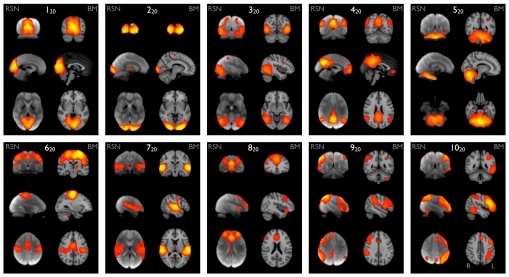
\includegraphics[scale=5]{smith_maps}
	\caption{Smith Maps ~\citep{Smith2009}. Borrowed from Smith (2009), this figure demonstrates the correspondence between reported activation coordinates (right column in each block) and resting state (left column in each block). Beta-series maps (decomposed via Independent Components Analysis) should also have high spatial correlations with the resting state components}
	\label{fig:smith_maps}
\end{figure}

After the beta-series maps are decomposed using ICA (for both congruent beta-series maps and incongruent beta-series maps), the components are predicted to show a high degree of spatial similarity with the components derived from Smith (2009) (Figure ~\ref{fig:smith_maps}).
Most importantly, there will be homologous components for the executive network (close to the cingulo-opercular network) and the left/right fronto-parietal networks.

\begin{figure}[H]%
	\centering
	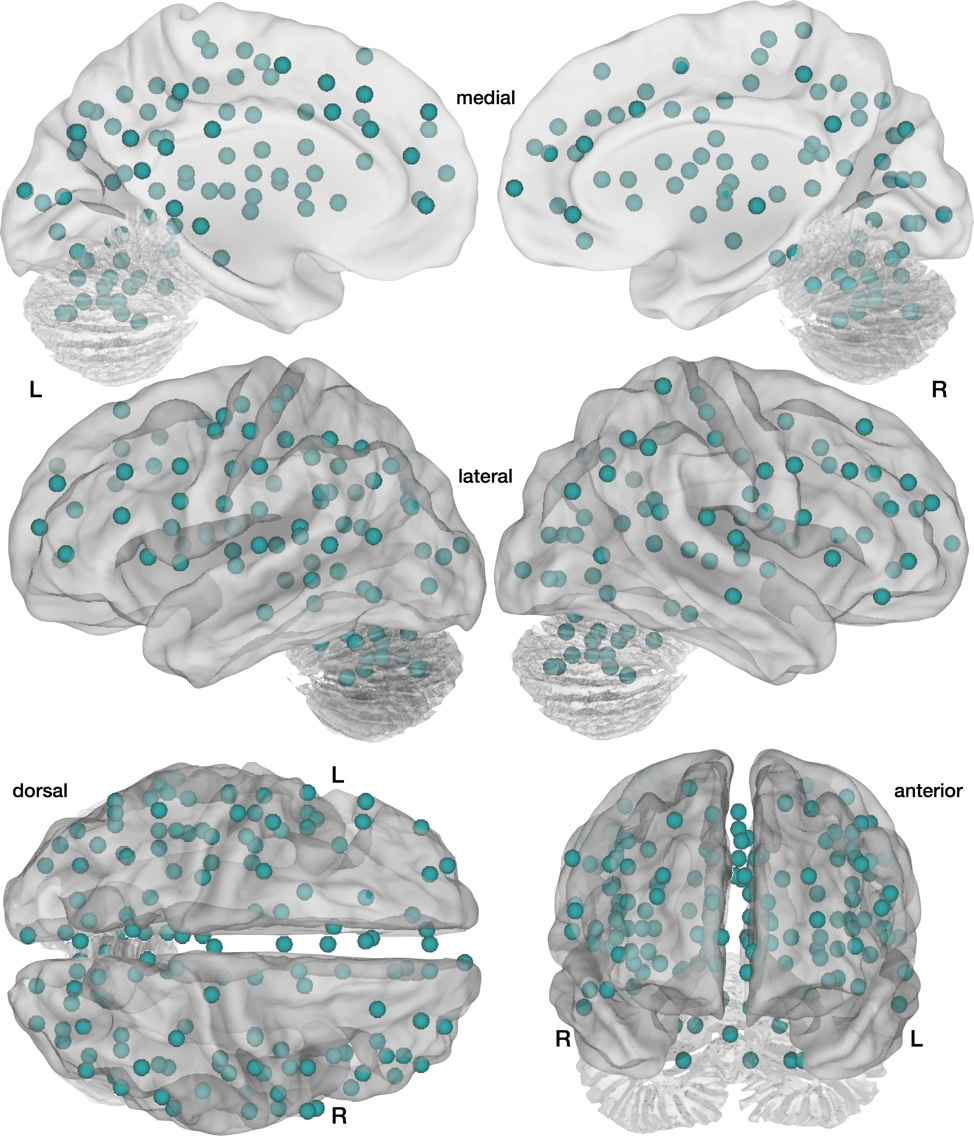
\includegraphics[scale=0.25]{dosenbach_rois}
	\caption{Dosenbach ROIs ~\citep{Dosenbach2010}. Pulled from the supplemental figures from Dosenbach (2010), The \href{https://github.com/nilearn/nilearn/blob/master/nilearn/datasets/data/dosenbach_2010.csv}{160 ROIs} were generated from 5 large meta-analyses. These ROIs will act as the seed regions for all beta-series correlations.}
	\label{fig:dosenbach_rois}
\end{figure}

Using the same beta-series maps, betas will be extracted and averaged from each ROI and correlated with every other ROI to produce a 160 x 160 symmetric matrix.
The predicted result is that for each condition (congruent and incongruent), the within network correlations for the fronto-parietal and cingulo-opercular network will be larger than the between network correlations.

\subsection{Preliminary Results}
The main result is that beta-series derived networks are similar to existing networks.
\begin{figure}[H]%
    \centering
    \newcounter{connum}
    \forloop{connum}{1}{\value{connum} < 21}{
    	\subfloat{{\includegraphics[width=2.0cm]{con_IC_\arabic{connum}} }}
    }
    \caption{Congruent Independent Components (Flanker). The Flanker task from the OpenFMRI dataset. Only the betas derived from the congruent trials were used to generate these components.}%

    \label{fig:con_ICs}%
\end{figure}

\begin{figure}[H]%
    \centering
    \newcounter{incnum}
    \forloop{incnum}{1}{\value{incnum} < 21}{
    	\subfloat{{\includegraphics[width=2.0cm]{inc_IC_\arabic{incnum}} }}
    }
    \caption{Incongruent Independent Components (Flanker). The Flanker task from the OpenFMRI dataset. Only the betas derived from the incongruent trials were used to generate these components.}%
    \label{fig:inc_ICs}%
\end{figure}

Decomposing the slow event related Flanker task with ICA presented 

\begin{figure}[H]%
	\centering
	\subfloat[congruent matrix]{{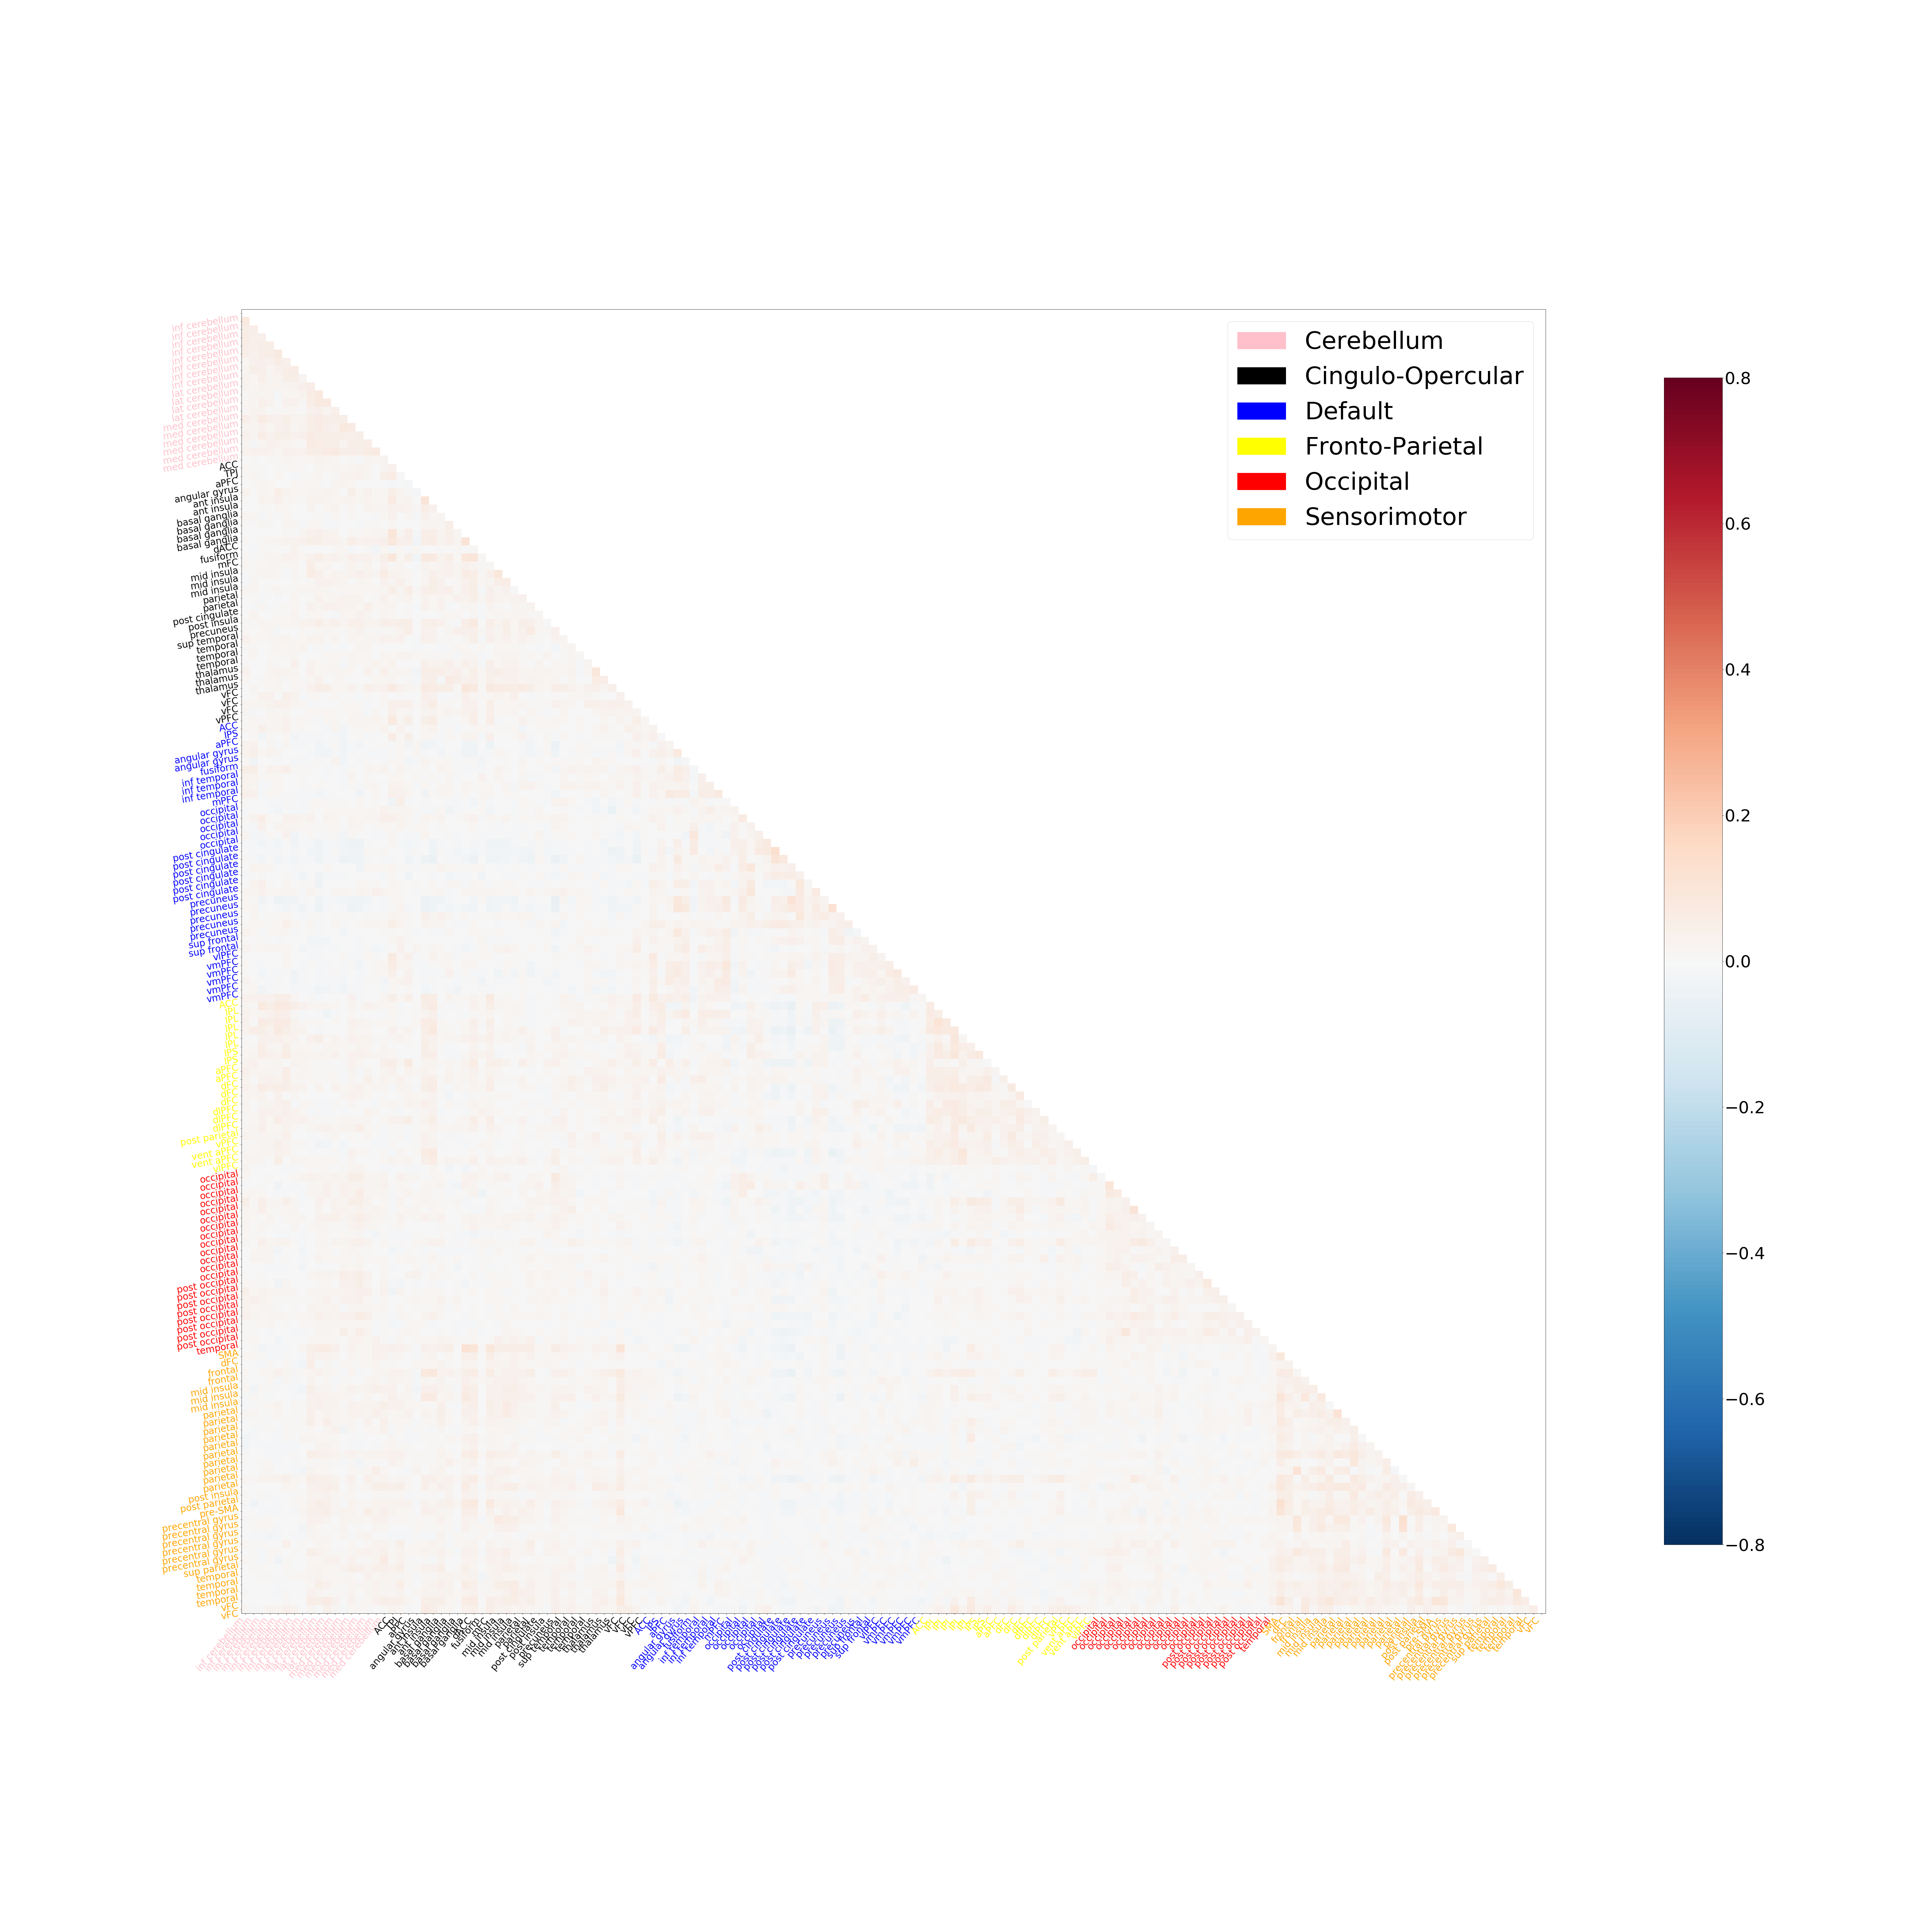
\includegraphics[width=0.5\linewidth]{congruent_dosenbach_flanker_matrix}}}
	\subfloat[incongruent matrix]{{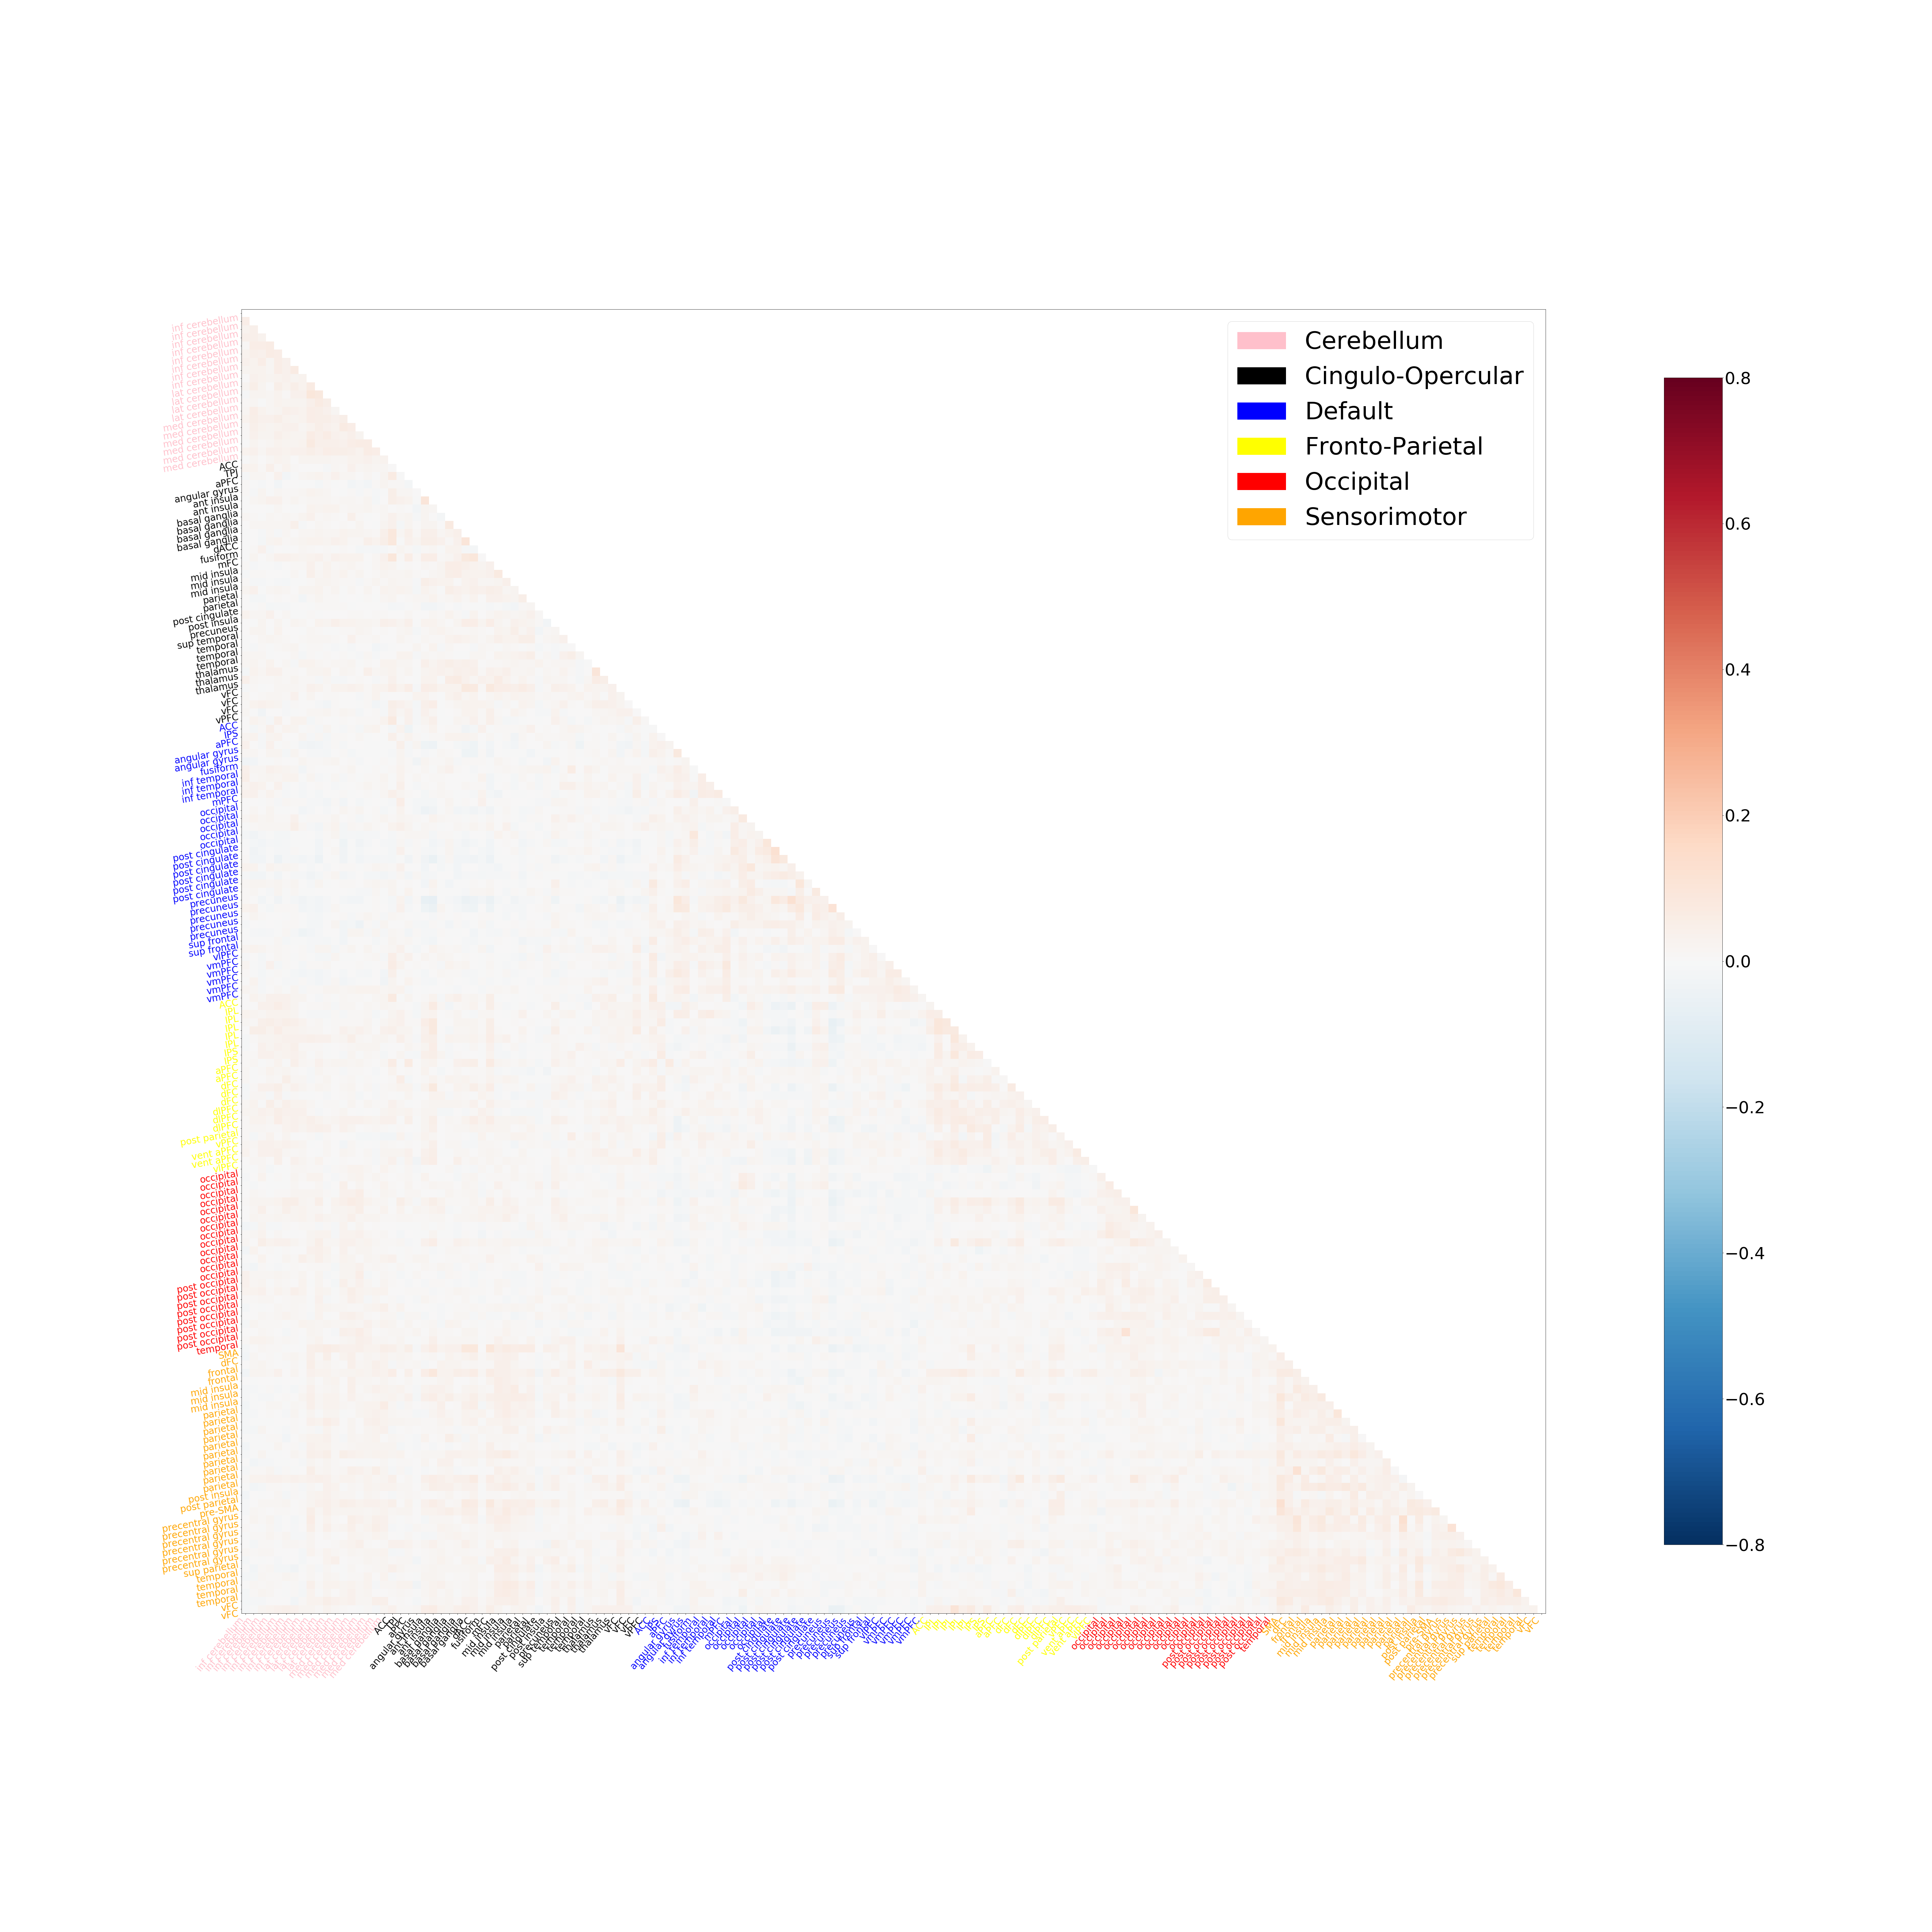
\includegraphics[width=0.5\linewidth]{incongruent_dosenbach_flanker_matrix}}}

	\subfloat[congruent connectome]{{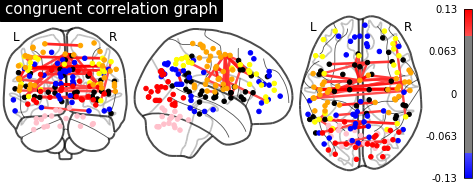
\includegraphics[width=0.5\linewidth]{congruent_dosenbach_flanker_connectome}}}
	\subfloat[incongruent connectome]{{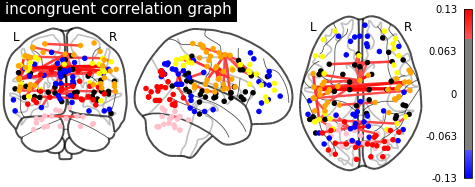
\includegraphics[width=0.5\linewidth]{incongruent_dosenbach_flanker_connectome}}}

\caption{Beta-series Correlations with Dosenbach ROIs (Flanker). The Flanker task from the OpenFMRI dataset. The matrices and connectomes represent the same data. a and c represent Beta-series Correlations from congruent trials, whereas b and d represent Beta-series Correlations from incongruent trials. The red lines between spheres in the connectomes represent the top 0.3\% correlations in the data. Network identification is color coded in the legends in the matrices, the same coloring scheme is used in the connectomes.}
\label{fig:OpenfMRIFlanker}
\end{figure}

\begin{figure}[H]%
	\centering
	\subfloat[congruent matrix]{{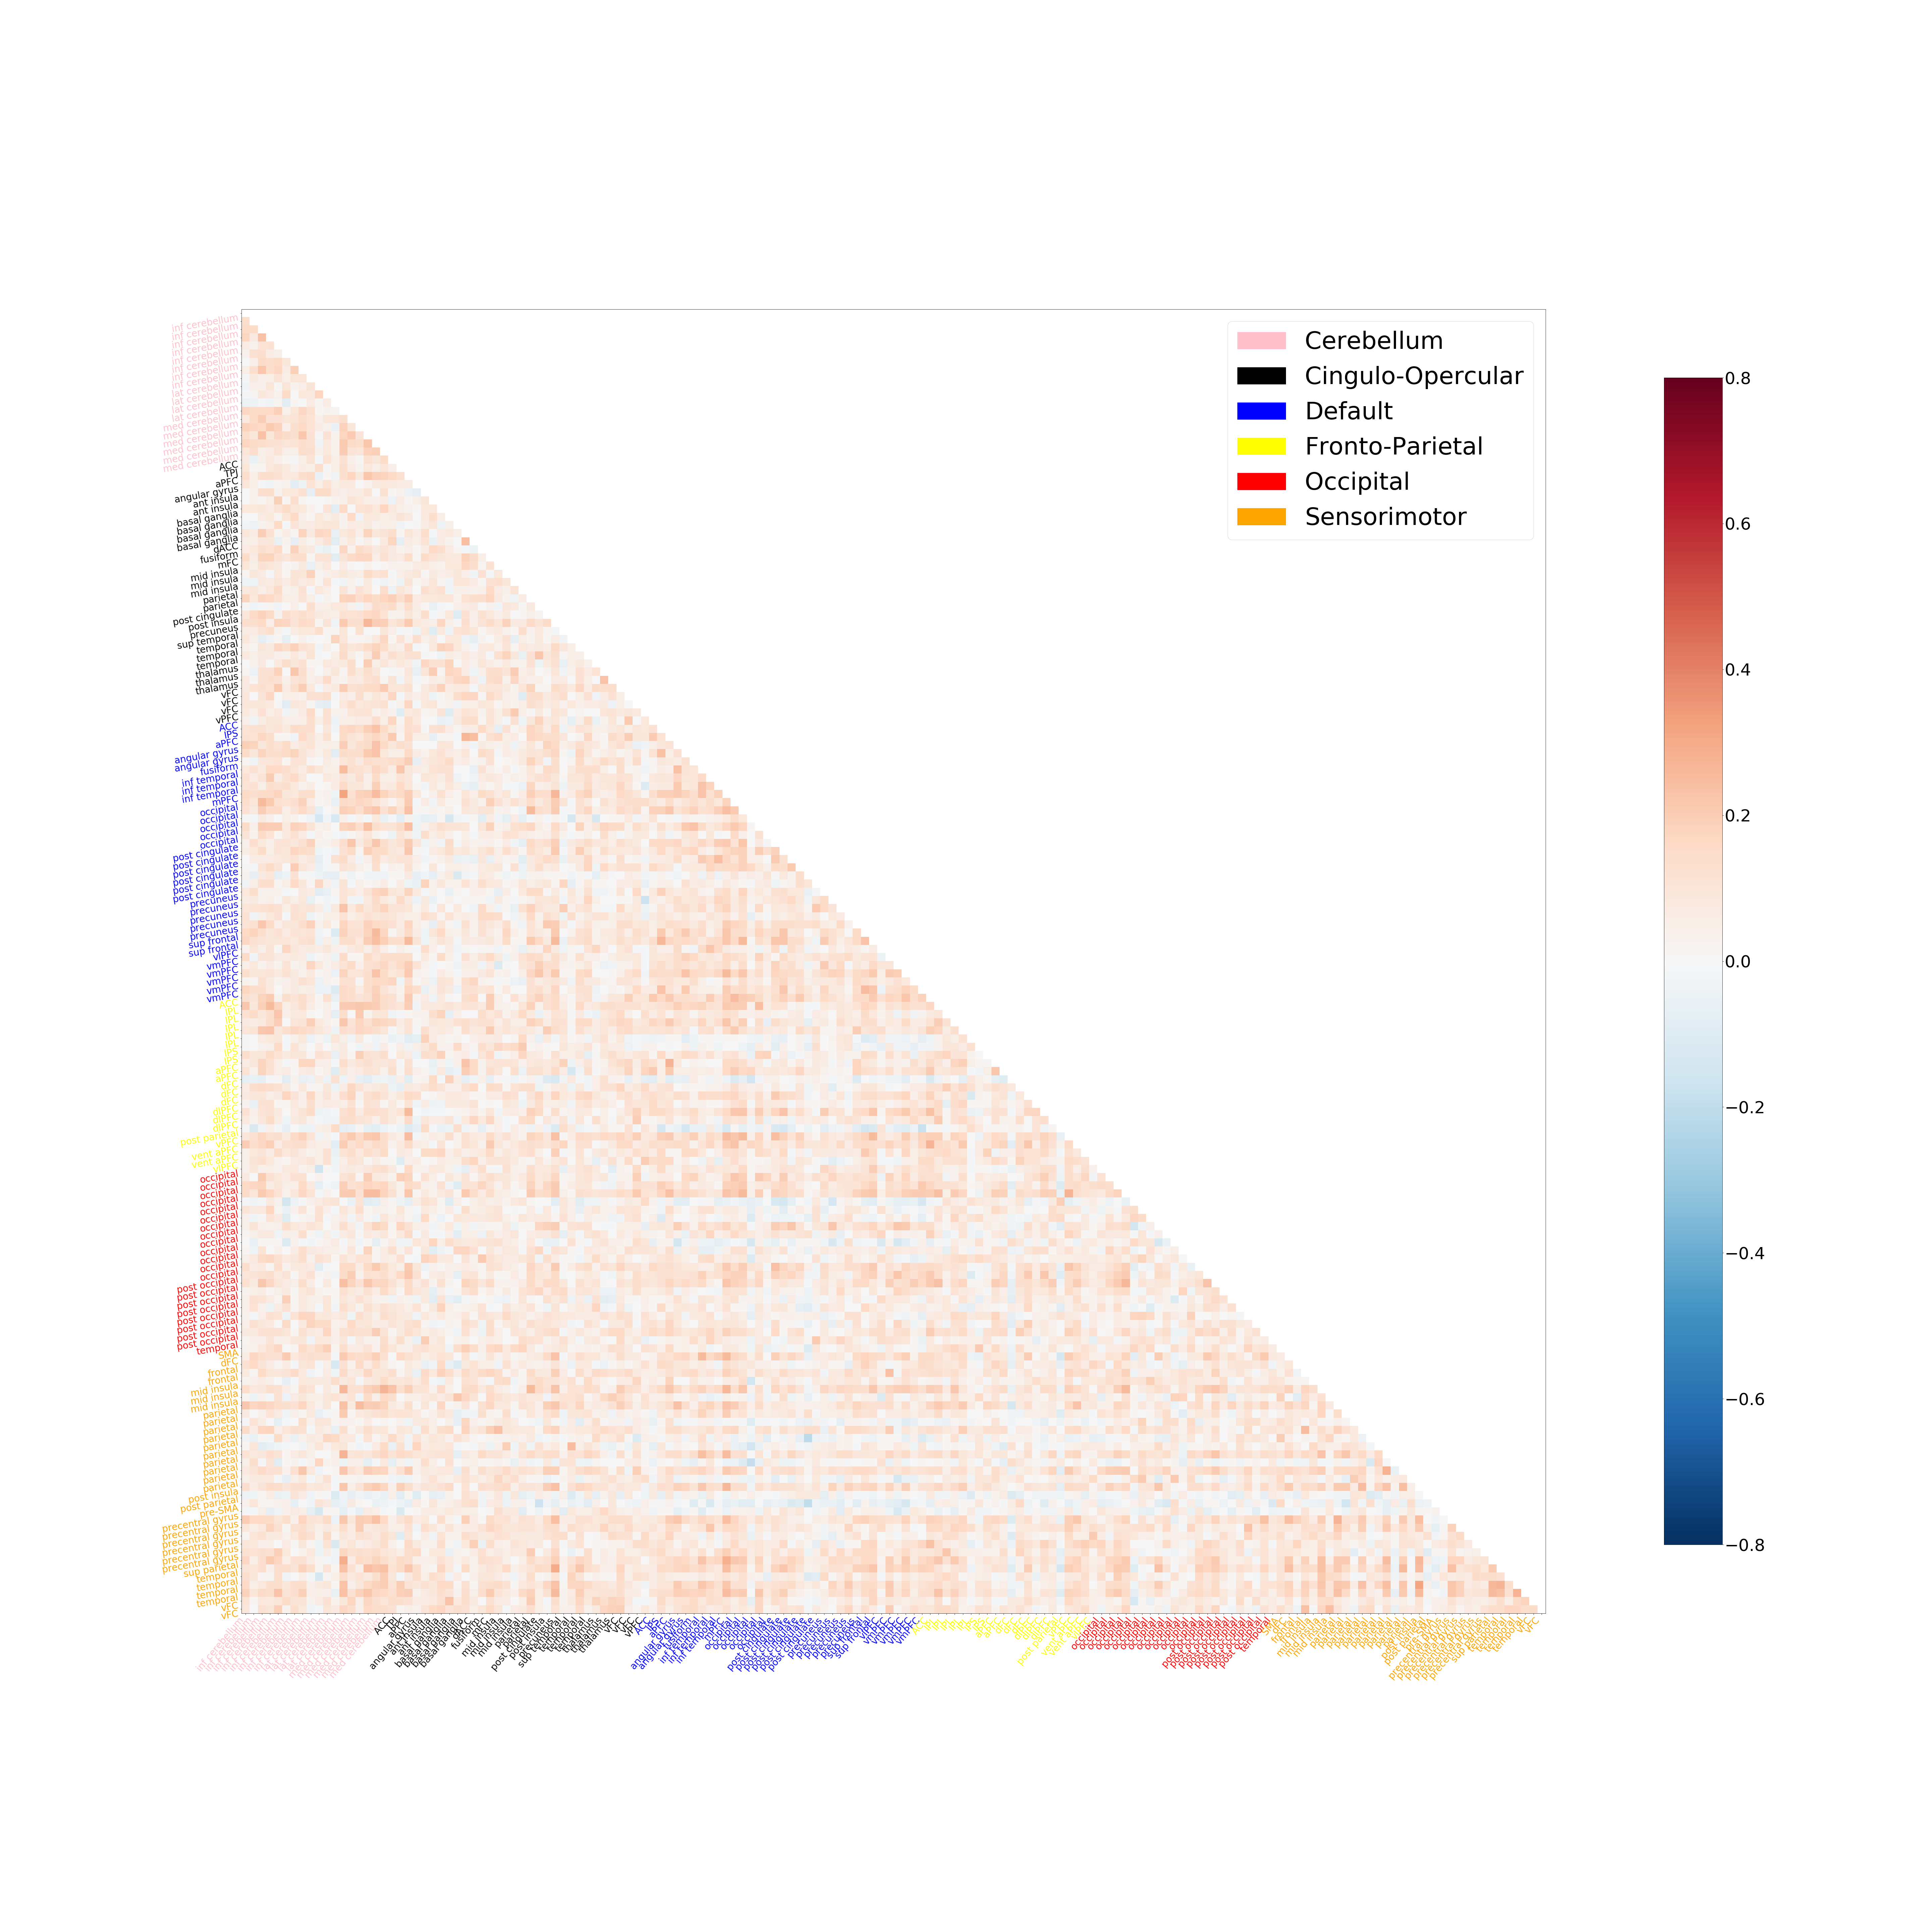
\includegraphics[width=0.5\linewidth]{congruent_dosenbach_simon_matrix}}}
	\subfloat[incongruent matrix]{{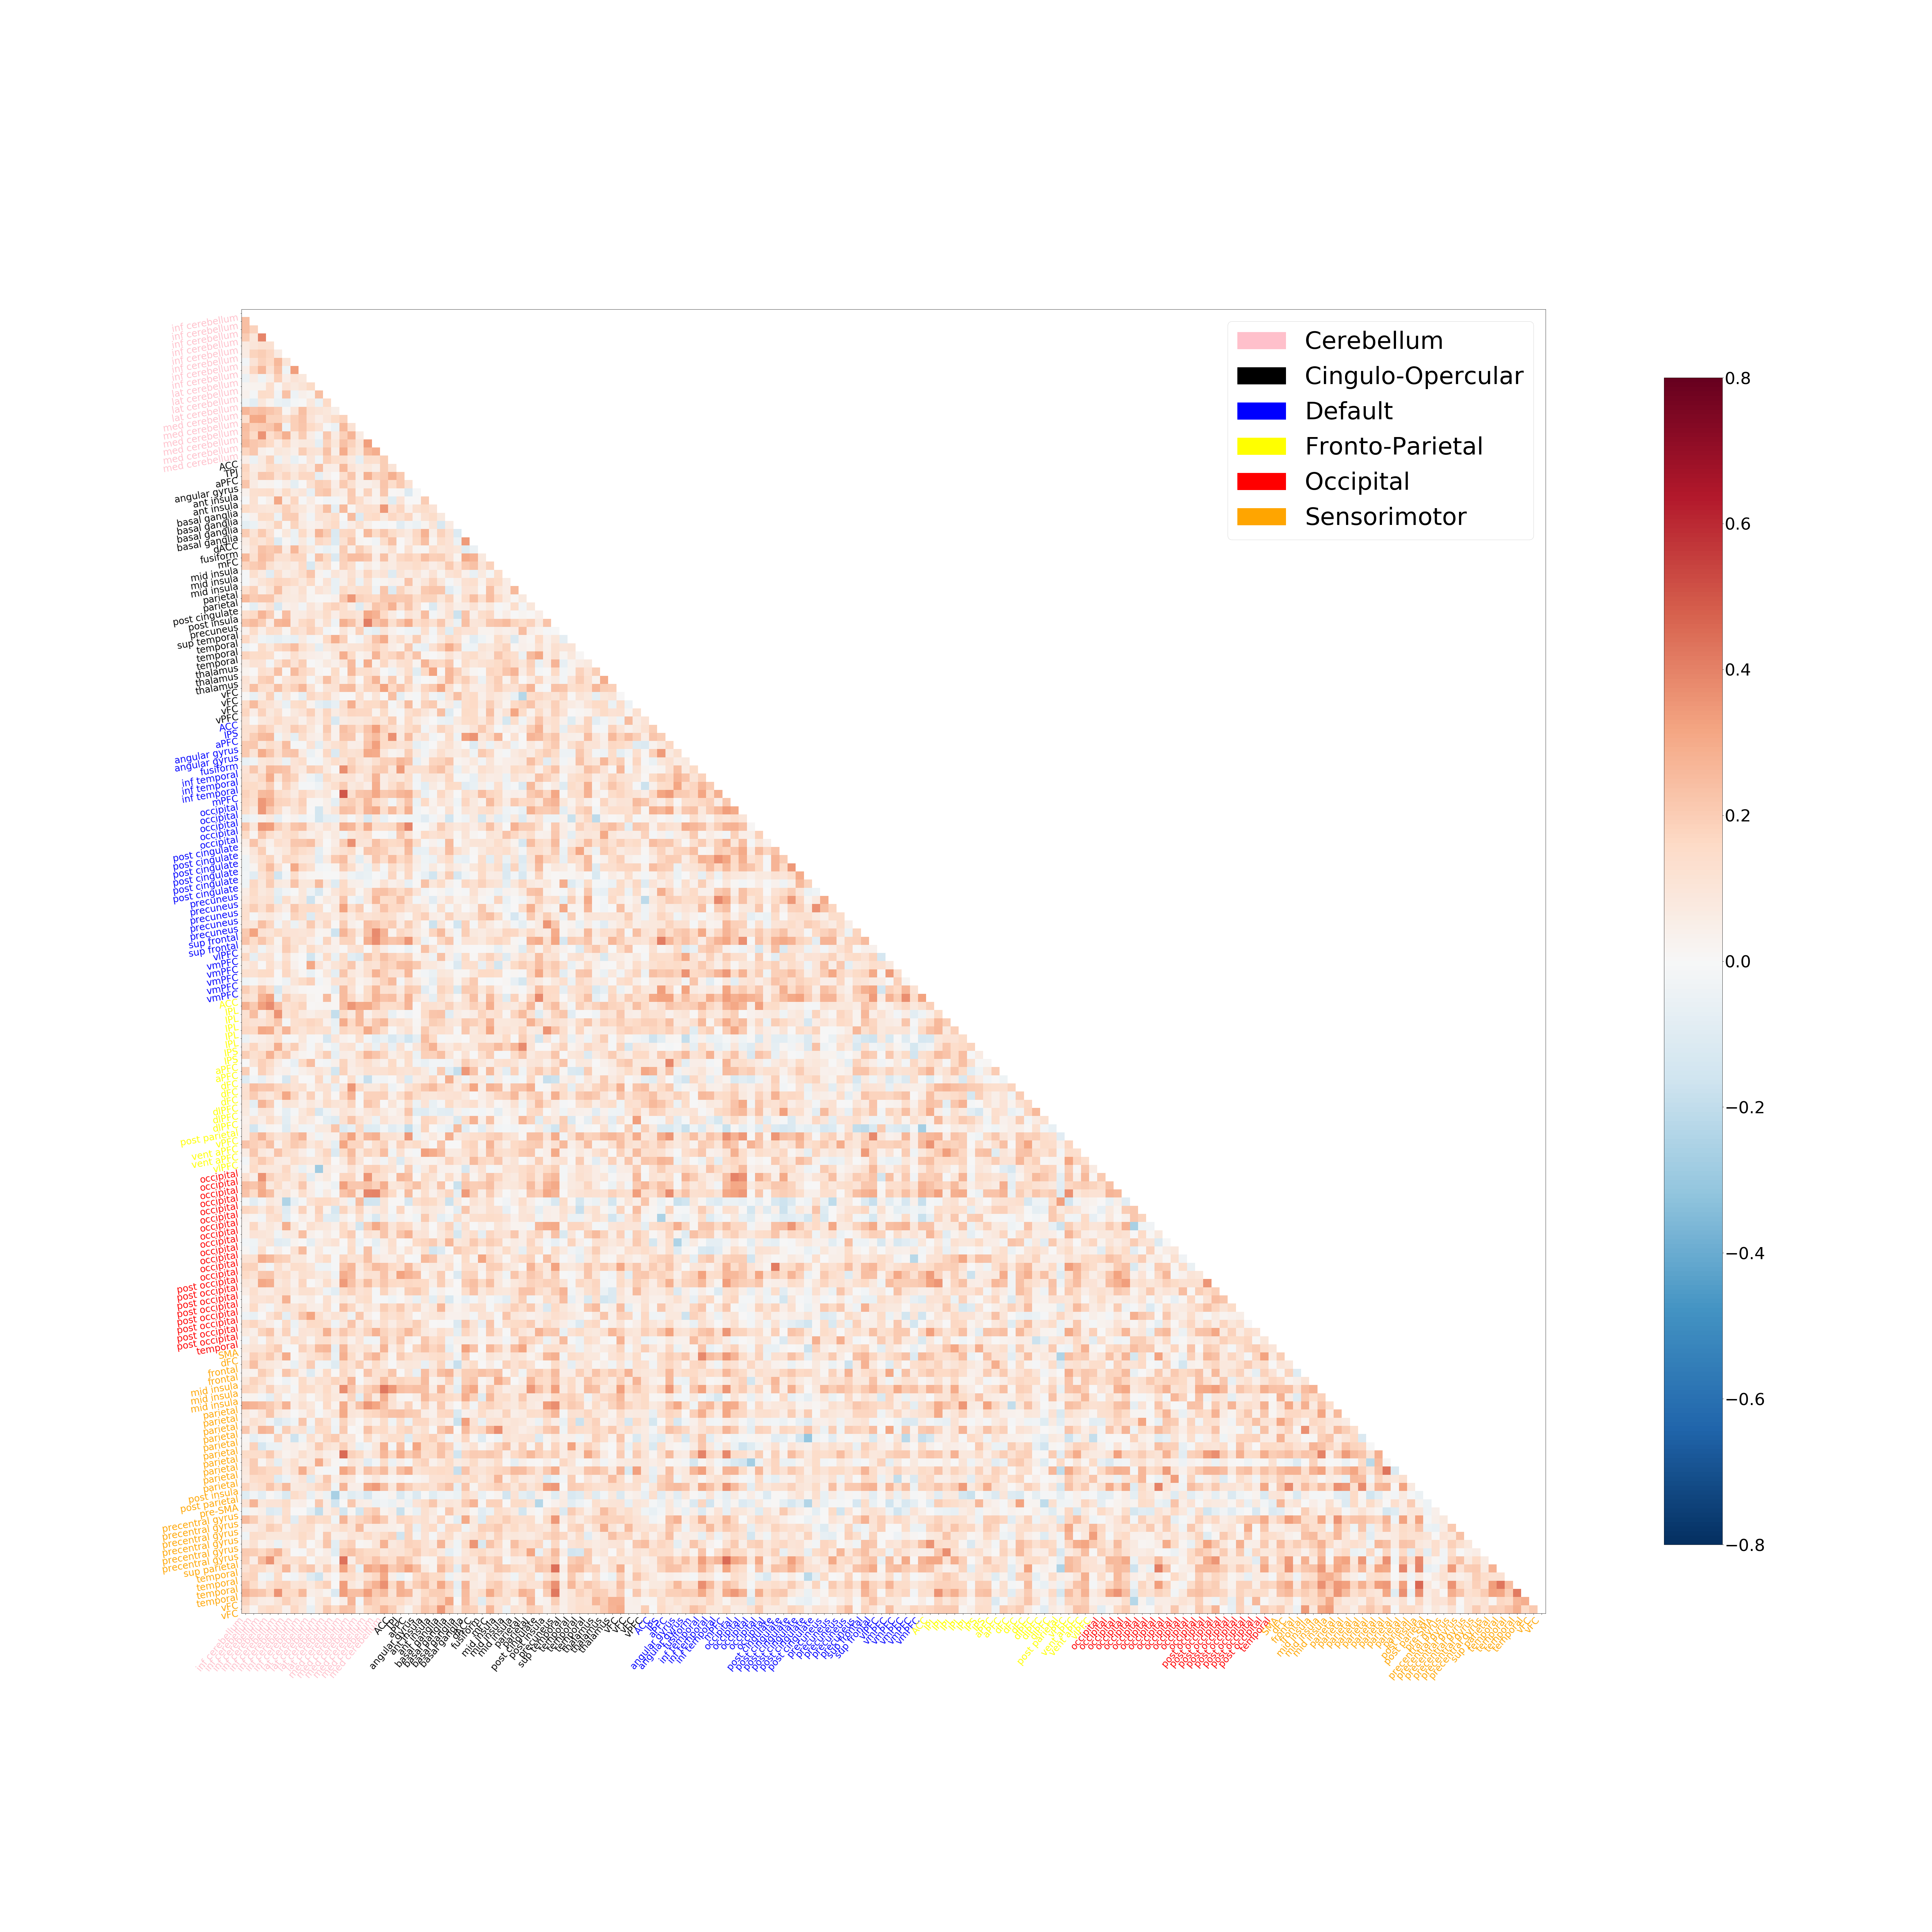
\includegraphics[width=0.5\linewidth]{incongruent_dosenbach_simon_matrix}}}

	\subfloat[congruent connectome]{{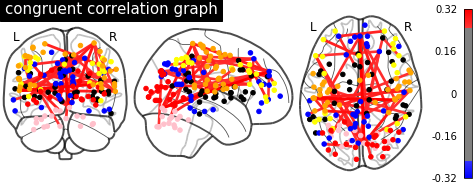
\includegraphics[width=0.5\linewidth]{congruent_dosenbach_simon_connectome}}}
	\subfloat[incongruent connectome]{{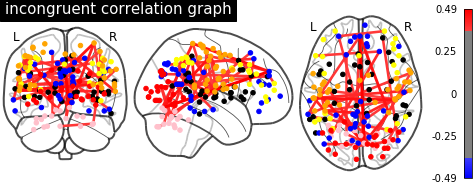
\includegraphics[width=0.5\linewidth]{incongruent_dosenbach_simon_connectome}}}

\caption{Beta-series Correlations with Dosenbach ROIs (Simon). The Simon task from the OpenFMRI dataset. The matrices and connectomes represent the same data. a and c represent Beta-series Correlations from congruent trials, whereas b and d represent Beta-series Correlations from incongruent trials. The red lines between spheres in the connectomes represent the top 0.3\% correlations in the data. Network identification is color coded in the legends in the matrices, the same coloring scheme is used in the connectomes.}
\label{fig:OpeFMRISimon}
\end{figure}

\section{Aim 2}
Once Beta-series correlations are established for use in a fast event-related design, the relationship between beta-series correlations and residual correlations will be determined.
Residual correlations (e.g. removing task activation before estimating functional connectivity) have been published before ~\citep{Fair2007,Cole2014,Bolt2017}.
However, previous derivations of residual correlations only removed the average task activation and did not account for trial-to-trial variability.
Additionally, those residual correlations have only been compared to resting networks, there has not been an investigation on how these residual correlations compare to task evoked correlations.

\subsection{Flanker Dataset}
\textit{Participants}: 58 participants (mean age 69.6 $\pm$ 3.5 (range 65-80), 36 females), without a history of psychiatric or neurological illness confirmed by psychiatric assessment. 
Only participants that scored 26 and above on the Montreal Cognitive Assessment (MoCA) were included for participation in order to exclude for cognitive impairment (mean = 27.7, range = 26-30). 
Additionally, participants were excluded if they weren't fluent in english, had a diagnosis of any dementia or neurodegenerative disease, any medical condition predisposing the participant to imminent functional decline.
Participants gave written informed consent as approved by the institutional review boards of the University of Iowa.
\newline
\textit{Flanker Task}: On each trial (inter-trial interval (ITI) was 2.72 seconds, with null events for jitter), five arrows were presented either all facing the same direction or with the central arrow facing the opposing direction.
The participant was instructed to only respond to the direction of the central arrow, responding only with their index fingers, (e.g. if the central arrow pointed left, participant should press with their left index finger and if the central arrow pointed right, the participant should press with their right index finger), as fast and as accurately as they could.
Participants performed 40 congruent, 40 incongruent, and 40 neutral trials (120 total), in a predetermined order (as per OptSeq) with 40 null trials (fixation only).
\newline
\textit{Data Acquisition}: Functional imaging data were acquired using a research dedicated Siemens Allegra 3.0 T scanner with an 8 channel Siemens head coil and a research dedicated GE Discovery 750W 3.0 T scanner with a 16 channel head coil.
They obtained 315 contiguous echo planar imaging (EPI) whole-brain functional volumes (SIEMENS: TR=2000 ms; TE=30 ms; flip angle=90\textdegree, 36 slices, matrix=64x64; FOV=384 mm; acquisition voxel size=3.44x3.44x4mm, GE: TR=2000 ms; TE=30 ms; flip angle=80\textdegree, 36 slices; matrix=64x64; FOV=192mm)
A high-resolution T1-weighted anatomical image was also acquired using a magnetization prepared gradient echo sequence (MPRAGE, TR=2300 ms; TE= 2.95 ms; TI=900 ms; flip angle=9\textdegree; 176 slices, FOV=256 mm, GE: BRAVO, TR=8.59 ms; TE: 3.38 ms; TI=450 ms; flip angle=12\textdegree; 252 slices, FOV=256 mm).
\subsection{Simon Dataset}
\textit{Participants}: 40 participants (mean age 64.3 $\pm$ 8.0, 19 females, range 50-80), without a history of psychiatric or neurological illness confirmed by psychiatric assessment. 
Participants gave written informed consent as approved by the institutional review boards of the University of Iowa.
\newline
\textit{Simon Task}: On each trial (inter-trial interval (ITI) was 2.50 seconds, with null events for jitter), an X or an O was presented on either to the left or the right of a central fixation cross.
The X and O were associated with a certain button press (either left or right index finger), and the pairing was counterbalanced across participants.
The participant was instructed to only respond to the X and O, irrespective of location, and also perform as quickly and as accurately as possible.
Participants performed 36 congruent and 36 incongruent trials (72 total), in a predetermined order (as per OptSeq) with 36 null trials (fixation only).
\newline
\textit{Data Acquisition}: Functional imaging data were acquired using a research dedicated GE Discovery 750W scanner, with a 32 channel head coil, located at the University of Iowa.
They obtained 151 contiguous echo planar imaging (EPI) whole-brain functional volumes (TR=2000 ms; TE=30 ms; flip angle=80\textdegree, 37 slices, matrix=64x64; FOV=192 mm; acquisition voxel size=3x3x4mm).
A high-resolution T1-weighted anatomical image was also acquired using a magnetization prepared gradient echo sequence (BRAVO, TR=8.464 ms; TE= 3.48 ms; TI=450 ms; flip angle=12\textdegree; 176 slices, FOV=256 mm).
\subsection{Analysis}
Betas will be extracted as they are in Aim 1.
Residual maps will derived by including one regressor per trial (convolved with a double gamma function) to remove the impact of trial-to-trial variations in direct response to the stimuli.
After the beta maps and the residual maps are centered (mean=0) and variance scaled to one, correlations will be performed between all extracted signals from ROIs (Figure ~\ref{fig:dosenbach_rois}), resulting in a 160x160 symmetric matrix for each participant.
Each participant will have their intra-network correlations averaged to have a singular value per network.
The average correlation from the fronto-parietal and cingulo-opercular networks across participants will be compared with one-tailed student's t-tests.
\subsection{Predictions}
We predict the intra-network connectivity will be greater in the fronto-parietal network than the cingulo-opercular network when performing beta-series correlations (Figures ~\ref{fig:predict_betaseries_ovr},~\ref{fig:predict_betaseries_spc}).
For residual correlations, on the other hand, we predict the intra-network connectivity will be greater in the cingulo-opercular network than the fronto-parietal network (Figure ~\ref{fig:predict_residuals}.
\begin{figure}[H]%
	\centering
	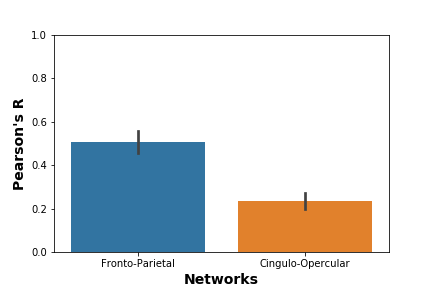
\includegraphics[scale=0.5]{predict_betaseries_ovr}
	\caption{Beta-series Correlation prediction (overall). The betas from the incongruent and congruent conditions are combined.}
	\label{fig:predict_betaseries_ovr}
\end{figure}

\begin{figure}[H]%
	\centering
	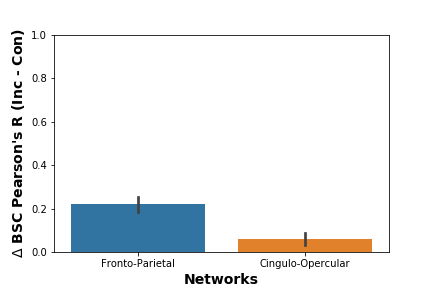
\includegraphics[scale=0.5]{predict_betaseries_spc}
	\caption{Beta-series Correlation prediction (condition specific). The average correlations derived from congruent trials are subtracted from the average correlations derived from incongruent trials.}
	\label{fig:predict_betaseries_spc}
\end{figure}

\begin{figure}[H]%
	\centering
	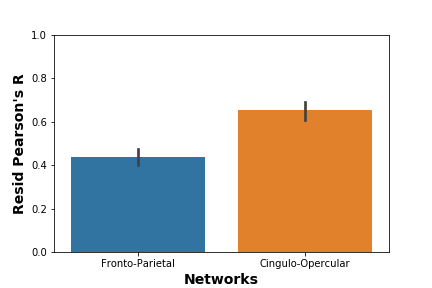
\includegraphics[scale=0.5]{predict_residuals}
	\caption{Residual prediction. The cingulo-opercular network demonstrates a stronger average within network correlations relative to the fronto-parietal network.}
	\label{fig:predict_residuals}
\end{figure}

\section{Aim 3}
The connection between the brain and behavior remains central to the field of neuroscience ~\citep{Krakauer2017}. 
And for good reason, while large curated datasets can tell us much about organization and mapping of the brain, how that organization applies to behavior is what drives theory and discovery. 
In the spirit of that idea, Aim 3 connects the cingulo-opercular and fronto-parietal networks with behavior. 
\subsection{Analysis}
The betas and residual maps will be calculated as explained in Aim 1 and Aim 2.
Reaction times from the Flanker and Simon Tasks will be averaged by condition (congruent and incongruent) per participant.
The congruency effect will be measured using the reaction time cost between incongruent and congruent conditions (e.g. incongruentRT $-$ congruentRT).
The congruency effect will be correlated with the average intra-network correlations for the fronto-parietal and cingulo-opercular networks across participants.
The strength of the correlations (network x behavior) will be compared with each other, such that the correlation between the average fronto-parietal intra-network correlation and the congruency effect will be compared to the average cingulo-opercular intra-network correlation and the congruency effect.
\subsection{Predictions}
We predict for beta-series analysis, the fronto-parietal average intra-network connectivity will correlate more strongly with congruency cost relative to the cingulo-opercular network's average intra-network connectivity correlation with congruency cost (Figures ~\ref{fig:predict_betaseries_rt_cost_ovr}, ~\ref{fig:predict_betaseries_rt_cost_spc}).
Whereas for residual analysis, the cingulo-opercular average intra-network connectivity will correlate more strongly with congruency cost relative to fronto-parietal network's average intra-network connectivity correlation with congruency cost (Figure ~\ref{fig:predict_residuals_rt_cost}).
\begin{figure}[H]%
	\centering
	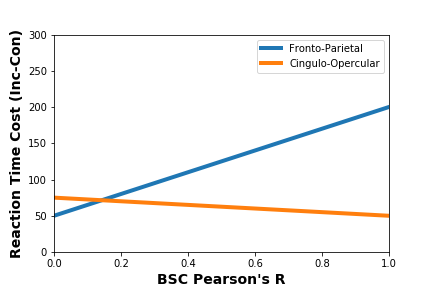
\includegraphics[scale=0.5]{predict_betaseries_rt_cost_ovr}
	\caption{Beta-series Correlation prediction (overall). The intra-network connectivity is averaged across conditions (congruent and incongruent). As reaction time cost increases, so does fronto-parietal average intra-network connectivity, consistent with reactive cognitive control. This relationship is slightly weaker then the condition specific measure because of the averaging across conditions.}
	\label{fig:predict_betaseries_rt_cost_ovr}
\end{figure}

\begin{figure}[H]%
	\centering
	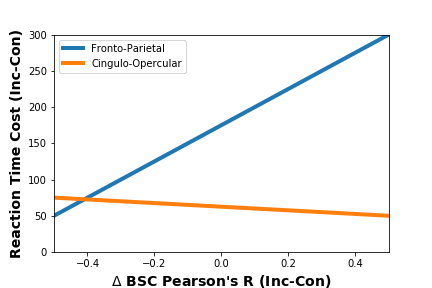
\includegraphics[scale=0.5]{predict_betaseries_rt_cost_spc}
	\caption{Beta-series Correlation prediction (condition specific). The intra-network connectivity is subtracted (incongruent $-$ congruent). As reaction time cost increases, so does fronto-parietal average intra-network connectivity, consistent with reactive cognitive control.}
	\label{fig:predict_betaseries_rt_cost_spc}
\end{figure}

\begin{figure}[H]%
	\centering
	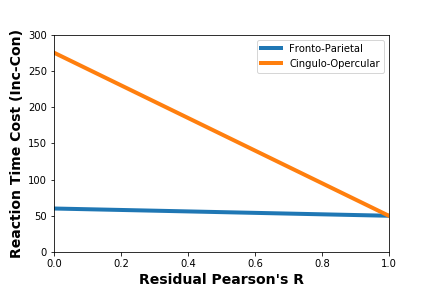
\includegraphics[scale=0.5]{predict_residuals_rt_cost_spc}
	\caption{Residual prediction. As reaction time cost increases, the cingulo-opercular average intra-network connectivity decreases, consistent with engagement of proactive control.}
	\label{fig:predict_residuals_rt_cost}
\end{figure}